% Template for PLoS
% Version 3.6 Aug 2022
%
% % % % % % % % % % % % % % % % % % % % % %
%
% -- IMPORTANT NOTE
%
% This template contains comments intended 
% to minimize problems and delays during our production 
% process. Please follow the template instructions
% whenever possible.
%
% % % % % % % % % % % % % % % % % % % % % % % 
%
% Once your paper is accepted for publication, 
% PLEASE REMOVE ALL TRACKED CHANGES in this file 
% and leave only the final text of your manuscript. 
% PLOS recommends the use of latexdiff to track changes during review, as this will help to maintain a clean tex file.
% Visit https://www.ctan.org/pkg/latexdiff?lang=en for info or contact us at latex@plos.org.
%
%
% There are no restrictions on package use within the LaTeX files except that no packages listed in the template may be deleted.
%
% Please do not include colors or graphics in the text.
%
% The manuscript LaTeX source should be contained within a single file (do not use \input, \externaldocument, or similar commands).
%
% % % % % % % % % % % % % % % % % % % % % % %
%
% -- FIGURES AND TABLES
%
% Please include tables/figure captions directly after the paragraph where they are first cited in the text.
%
% DO NOT INCLUDE GRAPHICS IN YOUR MANUSCRIPT
% - Figures should be uploaded separately from your manuscript file. 
% - Figures generated using LaTeX should be extracted and removed from the PDF before submission. 
% - Figures containing multiple panels/subfigures must be combined into one image file before submission.
% For figure citations, please use "Fig" instead of "Figure".
% See http://journals.plos.org/plosone/s/figures for PLOS figure guidelines.
%
% Tables should be cell-based and may not contain:
% - spacing/line breaks within cells to alter layout or alignment
% - do not nest tabular environments (no tabular environments within tabular environments)
% - no graphics or colored text (cell background color/shading OK)
% See http://journals.plos.org/plosone/s/tables for table guidelines.
%
% For tables that exceed the width of the text column, use the adjustwidth environment as illustrated in the example table in text below.
%
% % % % % % % % % % % % % % % % % % % % % % % %
%
% -- EQUATIONS, MATH SYMBOLS, SUBSCRIPTS, AND SUPERSCRIPTS
%
% IMPORTANT
% Below are a few tips to help format your equations and other special characters according to our specifications. For more tips to help reduce the possibility of formatting errors during conversion, please see our LaTeX guidelines at http://journals.plos.org/plosone/s/latex
%
% For inline equations, please be sure to include all portions of an equation in the math environment.  For example, x$^2$ is incorrect; this should be formatted as $x^2$ (or $\mathrm{x}^2$ if the romanized font is desired).
%
% Do not include text that is not math in the math environment. For example, CO2 should be written as CO\textsubscript{2} instead of CO$_2$.
%
% Please add line breaks to long display equations when possible in order to fit size of the column. 
%
% For inline equations, please do not include punctuation (commas, etc) within the math environment unless this is part of the equation.
%
% When adding superscript or subscripts outside of brackets/braces, please group using {}.  For example, change "[U(D,E,\gamma)]^2" to "{[U(D,E,\gamma)]}^2". 
%
% Do not use \cal for caligraphic font.  Instead, use \mathcal{}
%
% % % % % % % % % % % % % % % % % % % % % % % % 
%
% Please contact latex@plos.org with any questions.
%
% % % % % % % % % % % % % % % % % % % % % % % %

\documentclass[10pt,letterpaper]{article}
\usepackage[top=0.85in,left=2.75in,footskip=0.75in]{geometry}

% amsmath and amssymb packages, useful for mathematical formulas and symbols
\usepackage{amsmath,amssymb}

% Use adjustwidth environment to exceed column width (see example table in text)
\usepackage{changepage}

% textcomp package and marvosym package for additional characters
\usepackage{textcomp,marvosym}

% cite package, to clean up citations in the main text. Do not remove.
\usepackage{cite}

% Use nameref to cite supporting information files (see Supporting Information section for more info)
\usepackage{nameref,hyperref}

% line numbers
\usepackage[right]{lineno}

% ligatures disabled
\usepackage[nopatch=eqnum]{microtype}
\DisableLigatures[f]{encoding = *, family = * }

% color can be used to apply background shading to table cells only
\usepackage[table]{xcolor}

% array package and thick rules for tables
\usepackage{array}

% create "+" rule type for thick vertical lines
\newcolumntype{+}{!{\vrule width 2pt}}

% create \thickcline for thick horizontal lines of variable length
\newlength\savedwidth
\newcommand\thickcline[1]{%
  \noalign{\global\savedwidth\arrayrulewidth\global\arrayrulewidth 2pt}%
  \cline{#1}%
  \noalign{\vskip\arrayrulewidth}%
  \noalign{\global\arrayrulewidth\savedwidth}%
}

% \thickhline command for thick horizontal lines that span the table
\newcommand\thickhline{\noalign{\global\savedwidth\arrayrulewidth\global\arrayrulewidth 2pt}%
\hline
\noalign{\global\arrayrulewidth\savedwidth}}


% Remove comment for double spacing
%\usepackage{setspace} 
%\doublespacing

% Text layout
\raggedright
\setlength{\parindent}{0.5cm}
\textwidth 5.25in 
\textheight 8.75in

% Bold the 'Figure #' in the caption and separate it from the title/caption with a period
% Captions will be left justified
\usepackage[aboveskip=1pt,labelfont=bf,labelsep=period,justification=raggedright,singlelinecheck=off]{caption}
\renewcommand{\figurename}{Fig}

% Use the PLoS provided BiBTeX style
\bibliographystyle{plos2015}

% Remove brackets from numbering in List of References
\makeatletter
\renewcommand{\@biblabel}[1]{\quad#1.}
\makeatother



% Header and Footer with logo
\usepackage{lastpage,fancyhdr,graphicx}
\usepackage{epstopdf}
%\pagestyle{myheadings}
\pagestyle{fancy}
\fancyhf{}
%\setlength{\headheight}{27.023pt}
%\lhead{\includegraphics[width=2.0in]{PLOS-submission.eps}}
\rfoot{\thepage/\pageref{LastPage}}
\renewcommand{\headrulewidth}{0pt}
\renewcommand{\footrule}{\hrule height 2pt \vspace{2mm}}
\fancyheadoffset[L]{2.25in}
\fancyfootoffset[L]{2.25in}
\lfoot{\today}

%% Include all macros below

\newcommand{\lorem}{{\bf LOREM}}
\newcommand{\ipsum}{{\bf IPSUM}}

%% END MACROS SECTION


\begin{document}
\vspace*{0.2in}

% Title must be 250 characters or less.


\begin{flushleft}
{\Large
\textbf\newline{Multigroup nonnegative spatial factorization for genomic data} % Please use "sentence case" for title and headings (capitalize only the first word in a title (or heading), the first word in a subtitle (or subheading), and any proper nouns).
}
\newline
% Insert author names, affiliations and corresponding author email (do not include titles, positions, or degrees).
\\
Luis Chumpitaz-Diaz\textsuperscript{1,2},
Priyanka Shrestha, \textsuperscript{3},
Barbara E Engelhardt*\textsuperscript{2,4*}
\\
\bigskip
\textbf{1} Biophysics PhD Program, Stanford University, Stanford, CA, USA
\\
\textbf{2} Gladstone Institute of Data Science and Biotechnology, Gladstone Institutes, San Francisco, CA, USA
\\
\textbf{3} Department of Computer Science, Stanford University, Stanford, California, USA
\\
\textbf{4} Department of Biomedical Data Science, Stanford University, Stanford, California, USA
\\
\bigskip

% Insert additional author notes using the symbols described below. Insert symbol callouts after author names as necessary.
% 
% Remove or comment out the author notes below if they aren't used.
%
% Primary Equal Contribution Note
%\Yinyang These authors contributed equally to this work.

% Use the asterisk to denote corresponding authorship and provide email address in note below.
* barbarae@stanford.edu

\end{flushleft}
% Please keep the abstract below 300 words
% =========================


\section*{Abstract}
Spatially resolved transcriptomics (ST) techniques enable the study of gene expression within the spatial context of tissues, providing insights into tissue structure, cellular interactions, and disease progression. However, existing dimension reduction methods often overlook spatial information or struggle to distinguish spatial gene patterns from those driven by cell-type differences, limiting biological interpretability by convolving differences in gene expression patterns with differences in cell type proportions.
To address these challenges, we introduce multigroup nonnegative spatial factorization (MNSF), a scalable probabilistic framework that integrates spatial coordinates and cell-type labels into a unified matrix factorization model. By using multigroup Gaussian processes (MGGPs) as priors, our model captures complex spatial variation in a cell type specific way while enforcing nonnegativity to enhance interpretability.
We develop a variational inference framework for MGGPs that supports scalable optimization and improves the numerical stability of prior spatial models through Cholesky-based whitening and softplus-based constraints. Applied to complex ST datasets---including Slide-seqV2, Visium brain, and FFPE human colon---MNSF recovers sparse, interpretable spatial factors that reflect both spatial structure and cell-type-specific patterns in gene expression.
MNSF enables cell-type-aware spatial decompositions and offers a flexible foundation upon which to build more complex models. %Additionally, MNSF supports in silico cell-type perturbation to explore how changes in cellular composition might impact spatial gene expression. -- how?
MNSF provides a promising path for cell type specific hypothesis generation in developmental biology and disease.

\section*{Author summary}
Most current analysis methods for spatial transcriptomics either ignore spatial structure or fail to separate gene-driven spatial patterns from cell-type-driven differences. In this work, we develop a method that uses spatial coordinates and cell-type labels together to better uncover patterns of gene expression. Our approach, called Multigroup Nonnegative Spatial Factorization (MNSF), uses a machine learning technique known as a Gaussian process, which we extend to model both space and cell type in a unified framework using Multigroup Gaussian processes.

By applying our method to datasets from mouse brain, colon, and hippocampus tissues, we show that it produces clearer and more interpretable maps of where genes are active. This helps researchers understand how genes contribute to tissue organization and cell identity.

Beyond our specific model, this work introduces a general framework for incorporating spatial and group information into gene expression models. It can be extended to other applications, such as spatial PCA or other spatial factorization methods. This approach helps disentangle biological sources of variation and may support future analyses of how gene expression would change under different tissue or cell-type compositions.

\linenumbers

\section{Introduction}
Spatially-resolved transcriptomics (ST) techniques enable the measurement of gene expression while preserving spatial coordinates in tissue sections. This spatial information is crucial for understanding how gene activity varies across different tissue regions, how cells interact with their neighbors \cite{Verma2021-sj}, and how structure and function emerge in health and disease \cite{Moses2022-sw}. Such insights have been instrumental in the study of embryonic development \cite{Karaiskos2017-gf, Lohoff2022-ch, Hallou2025-sw}, tumor progression \cite{He2025-td, Zhang2024-wz}, and immune compartmentalization \cite{Kleshchevnikov2022-kw, Cable2022-cv}.

Dimension reduction techniques such as principal component analysis (PCA), factor analysis (FA) \cite{Bartholomew2011-vg}, and nonnegative matrix factorization (NMF) \cite{Lee1999-au} are commonly used to analyze high-dimensional single-cell RNA-sequencing (scRNA-seq) data \cite{Sun2019-kj, Wolf2018-sz, Butler2018-ej}. These methods can also be applied to ST datasets, but disregard spatial information altogether.

More recently, spatially aware models such as MEFISTO \cite{Velten2022-ci}, SpatialPCA \cite{Shang2022-ju}, and Nonnegative Spatial Factorization (NSF) \cite{Townes2023-it} use Gaussian processes (GPs) \cite{Seeger2004-gw} or related kernel-based priors to capture smooth spatial variation. MEFISTO uses an explicit GP formulation, while SpatialPCA uses a multivariate normal prior with spatial kernel-defined covariance—functionally similar to a GP. While these models recover spatial structure, their dense real-valued factors can be difficult to interpret. NSF improves interpretability by enforcing nonnegativity via exponentiated GP priors, yielding sparse, parts-based decompositions \cite{Townes2023-it}. However, none of these models explicitly incorporate cell-type information, limiting their ability to distinguish between spatial patterns that are gene-specific versus those driven by cell-type localization.

Classical non-spatial methods use transcriptomic profiles to infer cell types through dimensionality reduction, entirely independent of spatial context \cite{Butler2018-ej, Wolf2018-sz}. In contrast, spatial decomposition models like NSF \cite{Townes2023-it} or MEFISTO \cite{Velten2022-ci}, recover spatial gene expression patterns across tissues, but these can still be confounded by structured variation in cell-type abundance—especially when cell-type labels are not modeled explicitly. Meanwhile, methods such as cell2location \cite{Kleshchevnikov2022-kw} and C-SIDE \cite{Cable2022-cv} focus on estimating cell-type compositions across spatial locations using reference single-cell data and spatial information. However, these approaches are designed to recover cell types, not spatially structured gene expression patterns.

It is therefore important to distinguish between these goals. A \emph{cell type} is defined at specific spatial locations (i.e., individual cells or regions), while a \emph{spatial gene expression pattern}, as recovered by factorization models \cite{Townes2023-it, Velten2022-ci, Shang2022-ju}, is a structured signal distributed across the tissue. Without explicit modeling and consideration of cell types, spatial gene expression patterns can be misinterpreted. Often, it is impossible to know when spatial changes in gene expression are a function of expression changes within a cell type across the sample or changes in cell type frequencies across the sample, and deconvolving the impact of both types of changes on gene expression in spatial samples is an important task.

Clarifying the contribution of each source is essential for understanding how spatial regulation and cellular identity shape tissue architecture. For example, during embryonic development, positional information precedes cell identity: gradients of morphogens guide gene expression, differentiation, and tissue patterning before distinct cell types have formed. Methods such as DistMap \cite{Karaiskos2017-gf}, Lohoff et al. \cite{Lohoff2022-ch}, and Hallou et al. \cite{Hallou2025-sw} use spatial references and probabilistic models to localize scRNA-seq cells in developing embryos. In tumor microenvironments, spatial organization reflects interactions between malignant and immune cells, often forming structured niches. Methods like Starfysh \cite{He2025-td}, stKeep \cite{Zuo2024-mj}, and SpaTopic \cite{Zhang2024-wz} have uncovered spatial domains using expression patterns and graph-based decompositions. Similarly, in lymphoid and inflamed tissues, immune cells localize to compartments like B-cell follicles or T-cell zones. cell2location \cite{Kleshchevnikov2022-kw} models these cell-type distributions by integrating reference cell types with spatial transcriptomic profiles.

Despite this progress, many current spatial analysis models conflate gene- and cell-type-driven signals, making it difficult to determine whether observed spatial patterns are due to gene regulation or to cell-type composition \cite{Townes2023-it, Cable2022-cv}. This is particularly problematic because most ST datasets lack ground-truth cell-type labels and rely on unsupervised clustering or label transfer from scRNA-seq data \cite{Cable2022-cv, Sun2019-kj}. As a result, factorized spatial components may reflect gradients in cell-type abundance rather than gene-specific spatial programs. Such signals may appear to reflect gene-specific regulation when they are in fact driven by the spatial distribution of cell types across the tissue. Conversely, they may be attributed to the presence of particular cell types when the underlying variation is due to spatially structured expression of individual genes or gene programs, independent of cell identity. In many cases, spatial patterns reflect a combination of both effects. Without models that jointly account for spatial position and cell-type structure, disentangling these sources of variation, and assigning biological meaning to them, remains a fundamental challenge.

In this work, we introduce Multigroup Nonnegative Spatial Factorization (MNSF), a scalable and interpretable factorization method for spatial transcriptomics. MNSF integrates both spatial coordinates and known or inferred cell-type labels into a unified framework using Multigroup Gaussian Processes (MGGPs) \cite{Li2021-fv}. Unlike standard GPs, MGGPs enable the modeling of structured variation across multiple groups (e.g., cell types) while sharing statistical strength across the spatial domain.

Our method extends the NSF framework by replacing its GP prior with a multigroup GP prior over spatial factors~\cite{li2025bayesian}. This modification allows MNSF to model cell-type-specific spatial variation while preserving the interpretability and sparsity of nonnegative factorizations. We develop a variational inference framework for MGGPs, leveraging Cholesky-based whitening to improve numerical stability and scalability. This framework is general-purpose and can be applied to other spatial models such as SpatialPCA or any other latent variable GP model.

To ensure efficient optimization, we initialize the model with standard NMF and apply stochastic variational inference (SVI)
\cite{Blei2017-ed}, enabling application to large datasets with hundreds of thousands of spatial locations. % this isn't true anymore. also, this is methods, not introduction. I would move this last sentence to methods.
Furthermore, MNSF supports \emph{in silico} perturbation experiments and studies of cellular plasticity by allowing researchers to manipulate cell-type labels and observe the resulting predicted spatial transcriptomics patterns, providing a powerful direction for future hypothesis testing in spatial biology.
MNSF addresses key limitations of current spatial factorization methods by identifying spatial patterns in gene expression levels that are specific to cell type within a nonnegative, scalable, and interpretable probabilistic model. MNSF enables the disentanglement of gene- and cell-type-driven spatial patterns and offers a flexible framework that can be extended to a broad class of models for spatial transcriptomics.

\clearpage
\section{Materials and methods}

% ----------------------------
% 2.1 Background
% ----------------------------
\subsection{Non-Negative Spatial Factorization}\label{subsec21}


Non-negative spatial factorization is a method that expands Probabilistic Nonnegative Matrix Factorization (PNMF), a probabilistic version of NMF, by using a Gaussian process as prior, instead of a regular normal distribution. 
A similar method, MEFISTO, uses Gaussian Processes as a prior for FA \cite{Velten2022-ci} but encounters similar issues of FA and PCA, particularly in interpretability \cite{Townes2023-it}. 
PNMF provides a parts-based decomposition, which translated into NSF, provides interpretable non-negative factors belonging to genes in the dataset \cite{Townes2023-it}. 
The model is as follows:

\begin{eqnarray*}
y_{ij} &\sim& \text{Poisson}(\nu_i \lambda_{ij}) \\
\lambda_{ij} &=& \sum_{l=1}^L w_{jl} e^{f_{il}} \\
f_{il} &\sim& \text{GP}(f_{il} | \mu_l(x_i), K_l(x_i, X)).
\end{eqnarray*}
where:
\begin{itemize}
\item \( \nu_i \) is a per-cell normalization constant (e.g., total counts),
\item \( w_{jl} \) are nonnegative gene loadings, enforced via softplus transformation,
\item \( f_{il} \) are spatial latent factors drawn from a GP prior.
\end{itemize}

Here, the data consists of a cell by genes matrix of raw transcript counts \( Y \in \mathbb{R}^{N \times J} \) and spatial cell coordinates \( X \in \mathbb{R}^{N \times D} \).

\subsection{Multigroup Gaussian Processes}\label{subsec22}


Multigroup Gaussian Processes provide a family of positive-definite covariance kernel functions to perform Gaussian Process regression on multigroup data \cite{Li2021-fv}. The multidimensional inputs, \( X \in \mathbb{R}^{N \times D} \), also contain group labels, \( C=\{c_1,c_2,\ldots,c_N\} \), and outcomes \( Y \in \mathbb{R}^N \):

\[ p(Y|X, C_X; \theta) = \text{MGGP}(Y|X, C_X; K((X, C_X),(X, C_X))) \]

Where the kernel takes both the input and group label:

\[ K((x, c_j),(x', c_{j'})): X \times X \to \mathbb{R} \]

Various kinds and special cases of MGGPs exist. The simplest case is separate GPs (SGP), where \( K((x, c_j),(x', c_{j'}))=0 \), equivalent to training a separate GP per group \cite{Li2021-fv}. 
In our application to genomics, this approach is not useful as it means training a separate NSF model per cell type, resulting in zero correlation between cell types regardless of spatial distance. Union GP is equivalent to setting \( K((x, c_j),(x', c_{j'}))=K(x,x') \), meaning there is no group dependence, which is the current baseline of the NSF model. 
Separable MGGPs use the covariance function as the Kronecker product of two kernels: \( K((x, c_j),(x', c_{j'}))=K_1(x,x')K_2(c_i,c_{j'}) \). 
This is also known as multi-output and multitask Gaussian Processes \cite{Bonilla2007-gw}. 
However, these covariance functions can lead to "ridges" and discontinuities \cite{Stein2005-af,Li2021-fv}. 
For this work, we will use an inseparable isotropic MGGP analogous to the radial basis function (RBF) \cite{Li2021-fv} (see \ref{mggp}).

\subsection{Multigroup Non-Negative Spatial Factorization} \label{mggp}
Multigroup Nonnegative Spatial Factorization (MNSF) extends the Nonnegative Spatial Factorization (NSF) framework \cite{Townes2023-it} to incorporate both spatial coordinates and discrete group labels—typically cell types—into a unified generative model. MNSF models spatially structured latent factors using multigroup Gaussian processes (MGGPs) \cite{Li2021-fv}, enabling both (i) smooth signal sharing across related groups and (ii) structured differences between groups.

Relative to NSF (§\ref{subsec21}), the prior input is spatial coordinates \(X\), but also a vector of group labels \(C=\{c_1,\dots,c_N\}\); the GP prior now conditions on the pair \((x_i,c_i)\). This makes dimensionality reduction to operate on the gene-by-count matrix, spatial coordinates and cell-types (Fig.~\ref{fig1-overview}) .

\paragraph{Model.}
\begin{align*}
y_{ij} &\sim \text{Poisson}(\nu_i \lambda_{ij}), \\
\lambda_{ij} &= \sum_{l=1}^L w_{jl}\, e^{f_{il}}, \\
f_{il} &\sim \text{MGGP}\!\left(0,\, K_l\big((x_i, c_i), (X, C)\big)\right).
\end{align*}
Here, \(\nu_i\) and the nonnegative loadings \(w_{jl}\) are as in §\ref{subsec21}; the novelty is that the latent factors \(f_{il}\) are drawn from an MGGP prior that explicitly uses the group label \(c_i\).

\paragraph{Kernel.}
\begin{align*}
K\big((x, c), (x', c')\big)
= \sigma^2 \big(\alpha^2 d_{cc'}^2 + 1\big)^{-D/2}
  \exp\!\left(-\frac{\beta^2 \|x - x'\|^2}{\alpha^2 d_{cc'}^2 + 1}\right),
\end{align*}
where \(d_{cc'}\) encodes \textit{group (cell-type) distances} (e.g., \(d_{cc'}{=}0\) if \(c{=}c'\), \(d_{cc'}{=}1\) otherwise), \(\sigma\) is the marginal scale, \(\alpha\) controls the strength of difference between groups (cell-types), \(\beta\) is the spatial inverse length-scale, and \(D\) is the spatial dimension.


\begin{figure}[!h]
\includegraphics[width=0.98\linewidth]{MGGP_NSF_paper/Figure1.png}
\caption{ a) An outline of common dimension reduction algorithms and the corresponding sections of the dataset they operate. Both NSF and MEFISTO use the spatial positions to help factorize the cell by gene matrix. Our method expands NSF to also use cell clusters' labels, which can be cell types, tissue regions, etc. b) We show how spatial factors initialized with NMF become more sparse after training with stochastic variational inference (SVI), retaining the spatial component of the signal.}
\label{fig1-overview}
\end{figure}
% ----------------------------
% 2.2 Our method (MGGP in NSF) + inference
% ----------------------------
\subsection{MGGP Inference}
\subsubsection{Stochastic Variational Multigroup Gaussian Processes}

In order to perform inference on the NSF model using Multigroup Gaussian Processes, we first needed to build a variational strategy for such Gaussian Processes given the intractability of the NSF Poisson likelihood.
We follow similar strategies of previous stochastic variational Gaussian processes methods (SVGP) \cite{Hensman2013-xr,Salimbeni2017-ds,Townes2023-it}.
In particular, when using inducing points we also introduce \emph{inducing groups}: each inducing input \(z_m\) carries a label \(c_m\), so \((Z,C_Z)=\{(z_m,c_m)\}_{m=1}^M\); the labels \(C_Z\) are drawn from the observed group inputs (e.g., by sampling within each group).

\paragraph{Inducing construction.}
\begin{align*}
p(Y \mid X, C;\theta) &= \int p(Y \mid F)\, p(F \mid X, C;\theta)\, dF,\\
p(F \mid X, C;\theta) &= \int p(F \mid U, X, C, Z, C_Z;\theta)\, p(U \mid Z, C_Z;\theta)\, dU,\\
p(U \mid Z, C_Z;\theta) &= \mathcal{MGGP}\!\big(0, K\!\big((Z,C_Z),(Z,C_Z)\big)\big),
\end{align*}
where \((Z,C_Z)\) denote inducing locations and their associated inducing-group labels.

\paragraph{Variational objective.}
With \(q(F,U)=p(F \mid U,\cdot)\,q(U)\),
\begin{align*}
\mathcal{L} &= \mathbb{E}_{q(F)}\!\left[\log p(Y \mid F)\right]
 \;-\; \mathrm{KL}\!\big(q(U)\,\|\,p(U \mid Z, C_Z;\theta)\big)
\end{align*}


\paragraph{Whitening.}
Let \(U=L_Z g\) with \(g\sim\mathcal{N}(0,I)\) and \(L_ZL_Z^\top=K_{ZZ}\); work in the whitened space so the KL is closed-form and gradients are well-conditioned.

Full details of the ELBO derivation, closed-form expressions for the moments of \(q(F)\) used info the Poisson likelihood term, and the closed-form KL in the whitened space are provided in Appendix~S2–S4.





\subsubsection{Scaling Variational MGGPs}

While the MGGP variational framework enables stable training for our NSF model, in practice we are constrained by memory and can only use on the order of \(M{=}3{,}000\) inducing points during training—similar to the original NSF memory profile \cite{Townes2023-it}. 

\subsubsection*{Variational Nearest Neighbor Gaussian Processes}
VNNGPs offer an approximation of SVGP by using K-neast neighbors. In specfic a precision approximation for the inducing GP prior \cite{Wu2022-fd}.

\begin{align*}
p(U) &= p(U_1) \prod_{j=2}^{M} p(U_j | U_{1, \dots, j-1})\\
&\approx  \prod_{j=1}^{M} p(U_j | U_{n(j)})
\end{align*}

And they use the following approximation of the inducing variational distribution.
\begin{align*}
q(u) &= \prod_{i}^{M}\mathcal{N}\!\big(u_i; m_{u_i}, s_{u_i}\big),
\end{align*}


This works well for standard kernels on 1D inputs (near-banded precisions; Fig.~\ref{fig:precision-sparsity-regular}) but is ill-suited for MGGPs, where cross-group couplings produce non-diagonal block structure in the covariance and hence much denser precisions (Fig.~\ref{fig:precision-sparsity-mggp}). In MGGPs, these types of masking can induce ``separate MGGP'' behavior with ridges/discontinuities \cite{Li2021-mu}.

\begin{figure}[t]
  \centering
  % optional: small padding inside the box

  \includegraphics[width=0.9\linewidth]{MGGP_NSF_paper/mggp_files/2D_mggps.png}%
  

  \caption{Covariance matrices of MGGP with 2D inputs at various values of group difference and the sampling of each covariance matrix}
  \label{fig:precision-sparsity-regular}
\end{figure}





\begin{figure}[t]
  \centering

  \includegraphics[width=0.9\linewidth]{MGGP_NSF_paper/mggp_files/K400.png}%
  

  \caption{Covariance matrices of KNN MGGP at K=400 with 2D inputs, and the sampling of each covariance matrix}
  \label{fig:precision-sparsity-regular}
\end{figure}

Their variational strategy, reduces to an SVGP with diagonal \(S_u\), leading to underestimated posterior variances  (see Appendix). For our method, it is important to also approximate the non-diagonal variance of the inducing distribution, which pertains to "cell-to-cell" variance, and for MGGP it also captures "group-to-group" variance. 

\subsubsection*{Scalable neighborhood variational strategy.}
To account for "cell/group-to-cell/group" covariances, we approximate the full-rank precision via \emph{local} neighborhood precisions using an embedded factor \(L_u \in \mathbb{R}^{M\times K}\). For a neighborhood \(n(i)\),
\begin{align*}
\mathrm{inv}\!\big(S_{n(i)\,n(i)}\big) \;\approx\; \mathrm{inv}\!\big(L_{n(i)}L_{n(i)}^\top\big),
\end{align*}
and adopt the conditional variational structure
\begin{align*}
q(u) \;=\; \prod_i q\!\big(u_i \mid u_{n(i)}\big), 
\qquad
q\!\big(u_{n(i)}\big) \;=\; \mathcal{N}\!\big(m_{u_{n(i)}},\, L_{u_{n(i)}}L_{u_{n(i)}}^\top\big).
\end{align*}
This preserves expressive cross-cell (and cross-group) covariance within neighborhoods while remaining tractable. The resulting ELBO and the locally factorized KL (via a conditional chain rule) are derived in the Appendix, along with implementation details.




\subsection{Cell-type-conditional predictive posteriors}

Now that we have the variational construction, this yields a posterior GP that depends only on the corresponding inputs \((X_i, C_i)\) \cite{Salimbeni2017-ds}. 
\begin{align*}
q(F \mid X, C;\theta)
&= \int p(F \mid U, X, C, Z, C_Z;\theta)\; q(U)\, dU .
\end{align*}

Crucially, unlike a standard SVGP, the MGGP form permits predictions not only at new spatial locations but also under \emph{new or altered group labels}. Enabling us to ask questions such “what if the entire tissue were cell type A?”, turning the model into a practical predictive framework rather than stopping at factorization.


To quantify the dependence of spatial factors on cell-type labels, we perform these \textit{in silico} perturbation experiments. Given a trained model, we hold spatial coordinates \(X\) fixed and replace all labels \(C_X\) with a new configuration \(C_{X_{new}}\), e.g., setting all labels to a single cell-type.

\begin{align*}
q(F \mid X, C_X^{\mathrm{new}};\theta)
&= \int p(F \mid U, X, C_X^{\mathrm{new}}, Z, C_Z;\theta)\; q(U)\, dU .
\end{align*}


This allows us to generate posterior maps of spatial factors under controlled label perturbations, revealing whether each factor is:
\begin{itemize}
\item \emph{cell-type-specific} (strongly modulated by the cell-typeclabel),
\item \emph{shared} across cell types (invariant to cell-type label changes).
\end{itemize}

% ----------------------------
% 2.7 Datasets & preprocessing
% ----------------------------
\subsection*{Datasets and preprocessing}
We applied MNSF to three spatial transcriptomics datasets:
\begin{itemize}
\item \textbf{Slide-seqV2 hippocampus}: mouse hippocampal tissue with \(\sim 34{,}000\) spatial barcodes and 15 annotated cell types. Cell-type labels were transferred from scRNA-seq references.
\item \textbf{HuColonCa-FFPE MERFISH}: human colorectal cancer tissue with \(\sim 1\) million single-cell spatial profiles and \(\sim 50\) annotated cell types. For computational efficiency, we subsampled 100{,}000 cells while preserving cell-type diversity.
\item \textbf{Human liver (healthy vs.\ fibrotic)}: FFPE MERFISH liver samples across multiple patients and conditions. Samples were processed jointly and annotated using existing clustering and marker-based label transfer \cite{Cable2022-cv}.
\end{itemize}
All datasets were normalized using Squidpy \cite{Palla2022-vs} with total-count normalization and log transformation. Spatial coordinates were standardized to unit scale per axis, and \(k\)-means clustering within each label was used to initialize inducing point locations.

% ----------------------------
% 2.8 Baselines
% ----------------------------
\subsection*{Baseline methods}
We benchmarked MNSF against a range of existing methods for spatial decomposition, domain discovery, and spatial deconvolution:
\begin{itemize}
\item \textbf{PCA / FA}: non-spatial linear factor models \cite{Bartholomew2011-vg},
\item \textbf{NMF / PNMF}: nonnegative factorization without spatial priors \cite{Lee1999-au},
\item \textbf{NSF}: nonnegative spatial factorization using exponentiated GP priors \cite{Townes2023-it},
\item \textbf{MEFISTO}: GP factor model for spatial and temporal variation \cite{Velten2022-ci},

\end{itemize}

\begin{table}[!ht]
\begin{adjustwidth}{-2.25in}{0in}
\centering
\caption{{\bf Comparison of spatial transcriptomics methods.} Methods differ in whether they incorporate spatial information, account for cell types, use nonnegativity constraints, and in their modeling goals.}
\begin{tabular}{|l|c|c|c|l|l|}
\hline
\textbf{Method} & \textbf{Spatial} & \textbf{Cell-Type} & \textbf{Nonneg.} & \textbf{Inputs} & \textbf{Goal} \\ \thickhline
PCA / FA         & No  & No  & No  & Expression only & Linear projection \\
NMF / PNMF       & No  & No  & Yes & Expression only & Parts-based decomposition \\
SpatialPCA       & Yes & No  & No  & Expression + spatial & Spatial smoothing of latent space \\
NSF              & Yes & No  & Yes & Expression + spatial & Interpretable spatial decompositions \\
MEFISTO          & Yes & No  & No  & Expression + spatial & Continuous time/space variation \\
SpaTopic         & Yes & No  & Yes & Expression + graph & Domain discovery \\
FISHFactor       & Yes & No  & Yes & smFISH coords & Subcellular modeling \\
C-SIDE           & No  & Yes & Optional & Expression + covariates & Expression variation from metadata \\
cell2location    & Yes & Yes & No  & ST + scRNA-seq & Spatial deconvolution \\
DistMap          & Yes & No  & No  & scRNA-seq + spatial atlas & Map cells to embryo \\
Starfysh         & Yes & No  & No  & Expression + graph & Graph convolutional smoothing \\
stKeep           & Yes & No  & No  & Expression + kNN graph & Region segmentation \\
MNSF (Ours)      & Yes & Yes & Yes & Expression + spatial + cell-type & Spatial+cell-type decomposition \\
\hline
\end{tabular}
\label{table:method-comparison}
\end{adjustwidth}
\end{table}

\clearpage
\section{Results}

\subsection*{Overview and evaluation criteria}
We evaluate multigroup nonnegative spatial factorization (MNSF) across three representative spatial transcriptomics settings that differ in resolution and tissue organization: Slide-seqV2 hippocampus (near-cellular resolution), MERFISH FFPE human colon (single-cell resolution across a large field-of-view), and human liver (healthy versus fibrotic tissue). Across datasets, we assess (i) factor interpretability (sparsity and gene set coherence) in the sense of nonnegative factorization \cite{Townes2023-it}, (ii) spatial fidelity of factor maps (smoothness and correspondence to known anatomical domains), and (iii) cell-type specificity versus spatial sharing, by conditioning the posterior on cell-type labels (\emph{cell-type-conditional predictive posteriors}). We compare to spatial factorization baselines including NSF \cite{Townes2023-it}, MEFISTO \cite{Velten2022-ci}, and SpatialPCA \cite{Shang2022-ju}. % what about spatial LDA? are there others? NNMF?
\textit{[Placeholder: update cross-reference to Methods for the scalable nearest-neighbor approximation; remove VNNGP mention here if needed.]}

% --- Keep MERFISH colon and Liver sections as requested ---

\subsection*{MERFISH FFPE human colon: widespread labels enable global enrichment patterns}
We next applied VNNGP-MNSF to a large FFPE human colon MERFISH dataset with \(\sim\)50 cell types; to ensure tractable training, we subsampled 100{,}000 cells while maintaining cell-type diversity. In contrast to the hippocampus, many colon cell types are distributed across broader tissue extents. Under cell-type-conditional posteriors, MNSF revealed structured \emph{enrichment} and \emph{depletion} patterns spanning the colon mucosa (Fig~\ref{fig4a}–\ref{fig4e}), rather than the near-uniform depletion observed in Slide-seqV2. These maps aligned with expected epithelial–stromal compartmentalization and immune localization patterns reported in spatial literature \cite{Kleshchevnikov2022-kw, Cable2022-cv, Townes2023-it}.

Compared to NSF \cite{Townes2023-it}, MNSF produced factors whose spatial support better matched the distributions of specific cell types when conditioning, while retaining sparse loadings that facilitated gene-level interpretation (top genes concentrated on pathway-consistent sets; cf.\ \cite{Townes2023-it}). Relative to MEFISTO \cite{Velten2022-ci} and SpatialPCA \cite{Shang2022-ju}, MNSF’s nonnegativity yielded more localized, additive parts that were easier to relate to anatomic microdomains. These findings indicate that when labels are spatially widespread, MNSF learns cell-type-aware spatial functions whose conditional posteriors are biologically meaningful at the tissue scale.

\subsection*{Human liver: shared initialization enables comparison across healthy and fibrotic tissues}
To assess condition-specific remodeling, we analyzed human liver samples from healthy and fibrotic tissues. We first trained MNSF on pooled healthy samples and transferred the learned factors/loadings to initialize per-sample models, partially mitigating non-identifiability of NMF-like factorizations and enabling cross-sample tracking of factors.

Across replicates, several spatial factors were conserved in healthy tissue, mapping to canonical hepatic architecture (e.g., hepatocyte- and endothelial-enriched domains). In fibrotic samples, the same factors exhibited altered spatial domains and cell-type associations (Fig~\ref{fig7-liver}). Cell-type-conditional posteriors highlighted disease-specific shifts: hepatocyte-conditioned factors redistributed away from fibrotic tracts, while endothelial-conditioned factors showed patterns consistent with vascular remodeling (Fig~\ref{fig8-liver-posteriors}).

\subsection*{Benchmarking summary across datasets}
Across all tissues, MNSF matched or exceeded the spatial fidelity of GP-based baselines (MEFISTO \cite{Velten2022-ci}, SpatialPCA \cite{Shang2022-ju}) while preserving the sparse, parts-based interpretability of NSF \cite{Townes2023-it}. The principal advantages we observe are: (i) \textbf{disentanglement} of cell-type versus spatial signal via label-aware priors, (ii) \textbf{interpretability} from nonnegativity (more localized, additive factors), and (iii) \textbf{scalability} via the VNNGP approximation on large fields-of-view. \textit{[Placeholder: update to reference our scalable nearest-neighbor method instead of VNNGP if needed.]}

% ----------------------------
% Figures already provided in your material; kept as-is
% ----------------------------



\begin{figure}[!h]
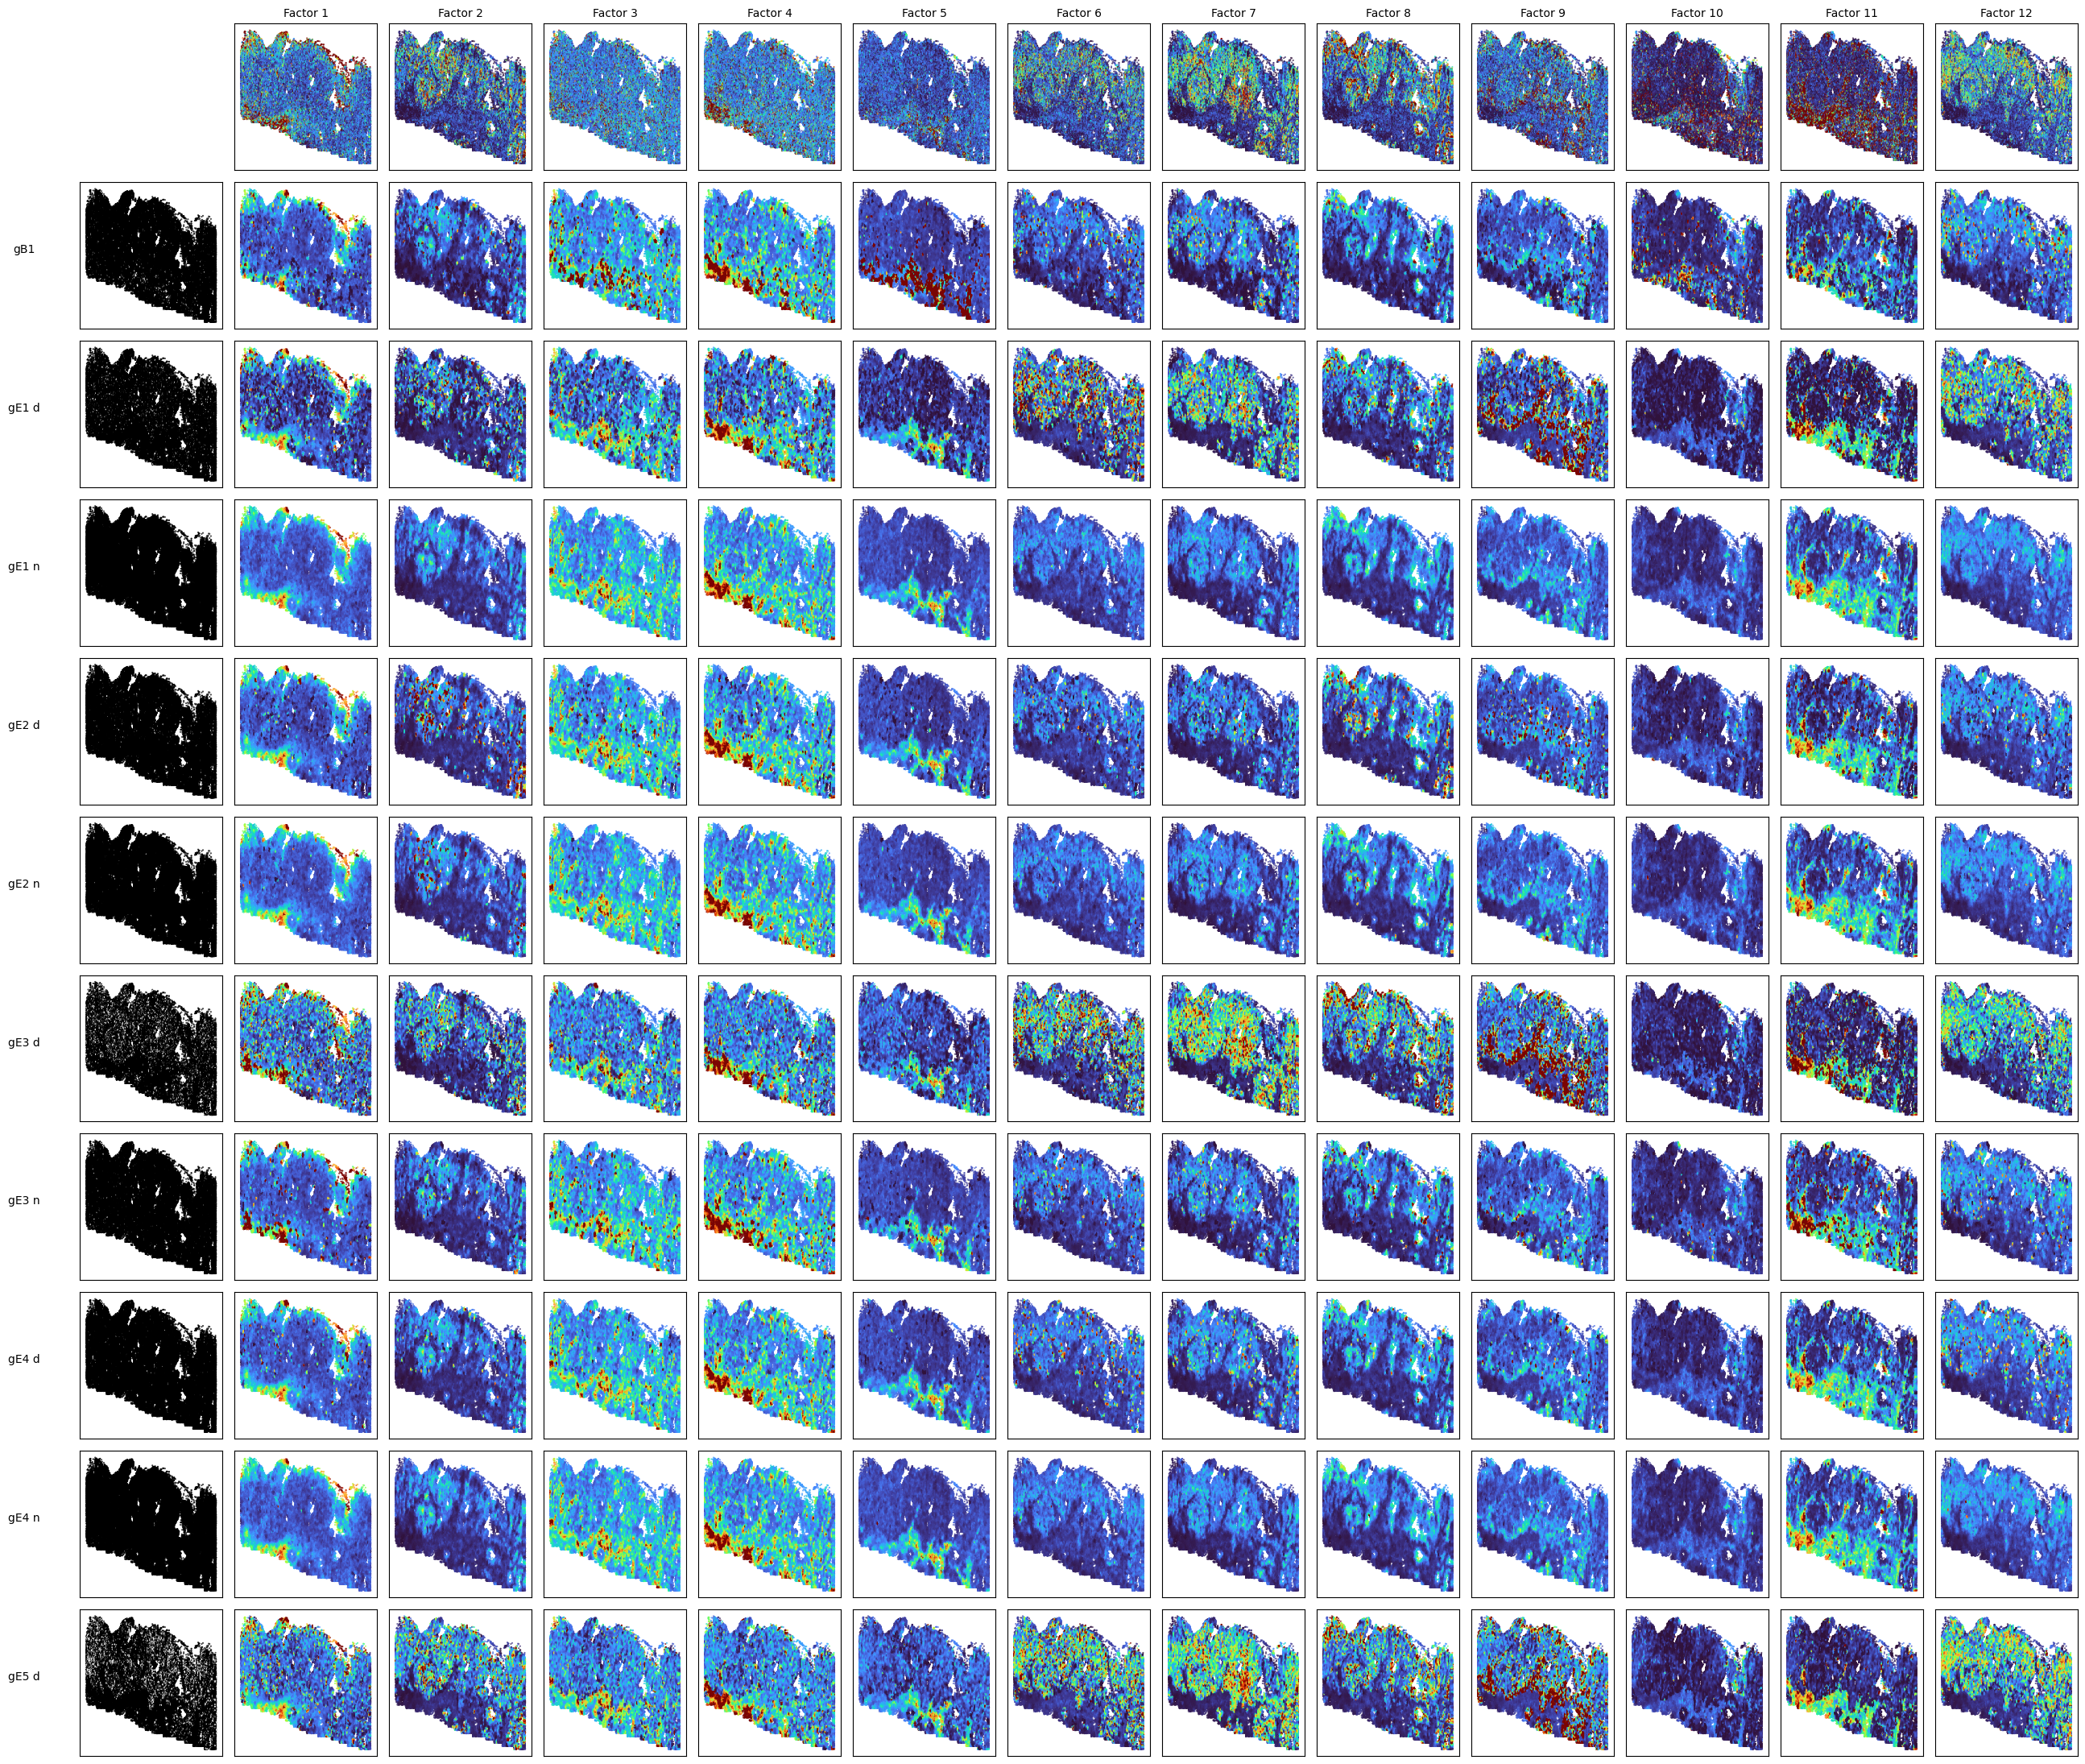
\includegraphics[width=0.98\linewidth]{MGGP_NSF_paper/HuColonCa-FFPE/posterior_1.png}
\caption{{\bf MERFISH CRC slices to show results from NSF versus MGNSF.}XXX }
\label{fig4a}
\end{figure}

\begin{figure}[!h]
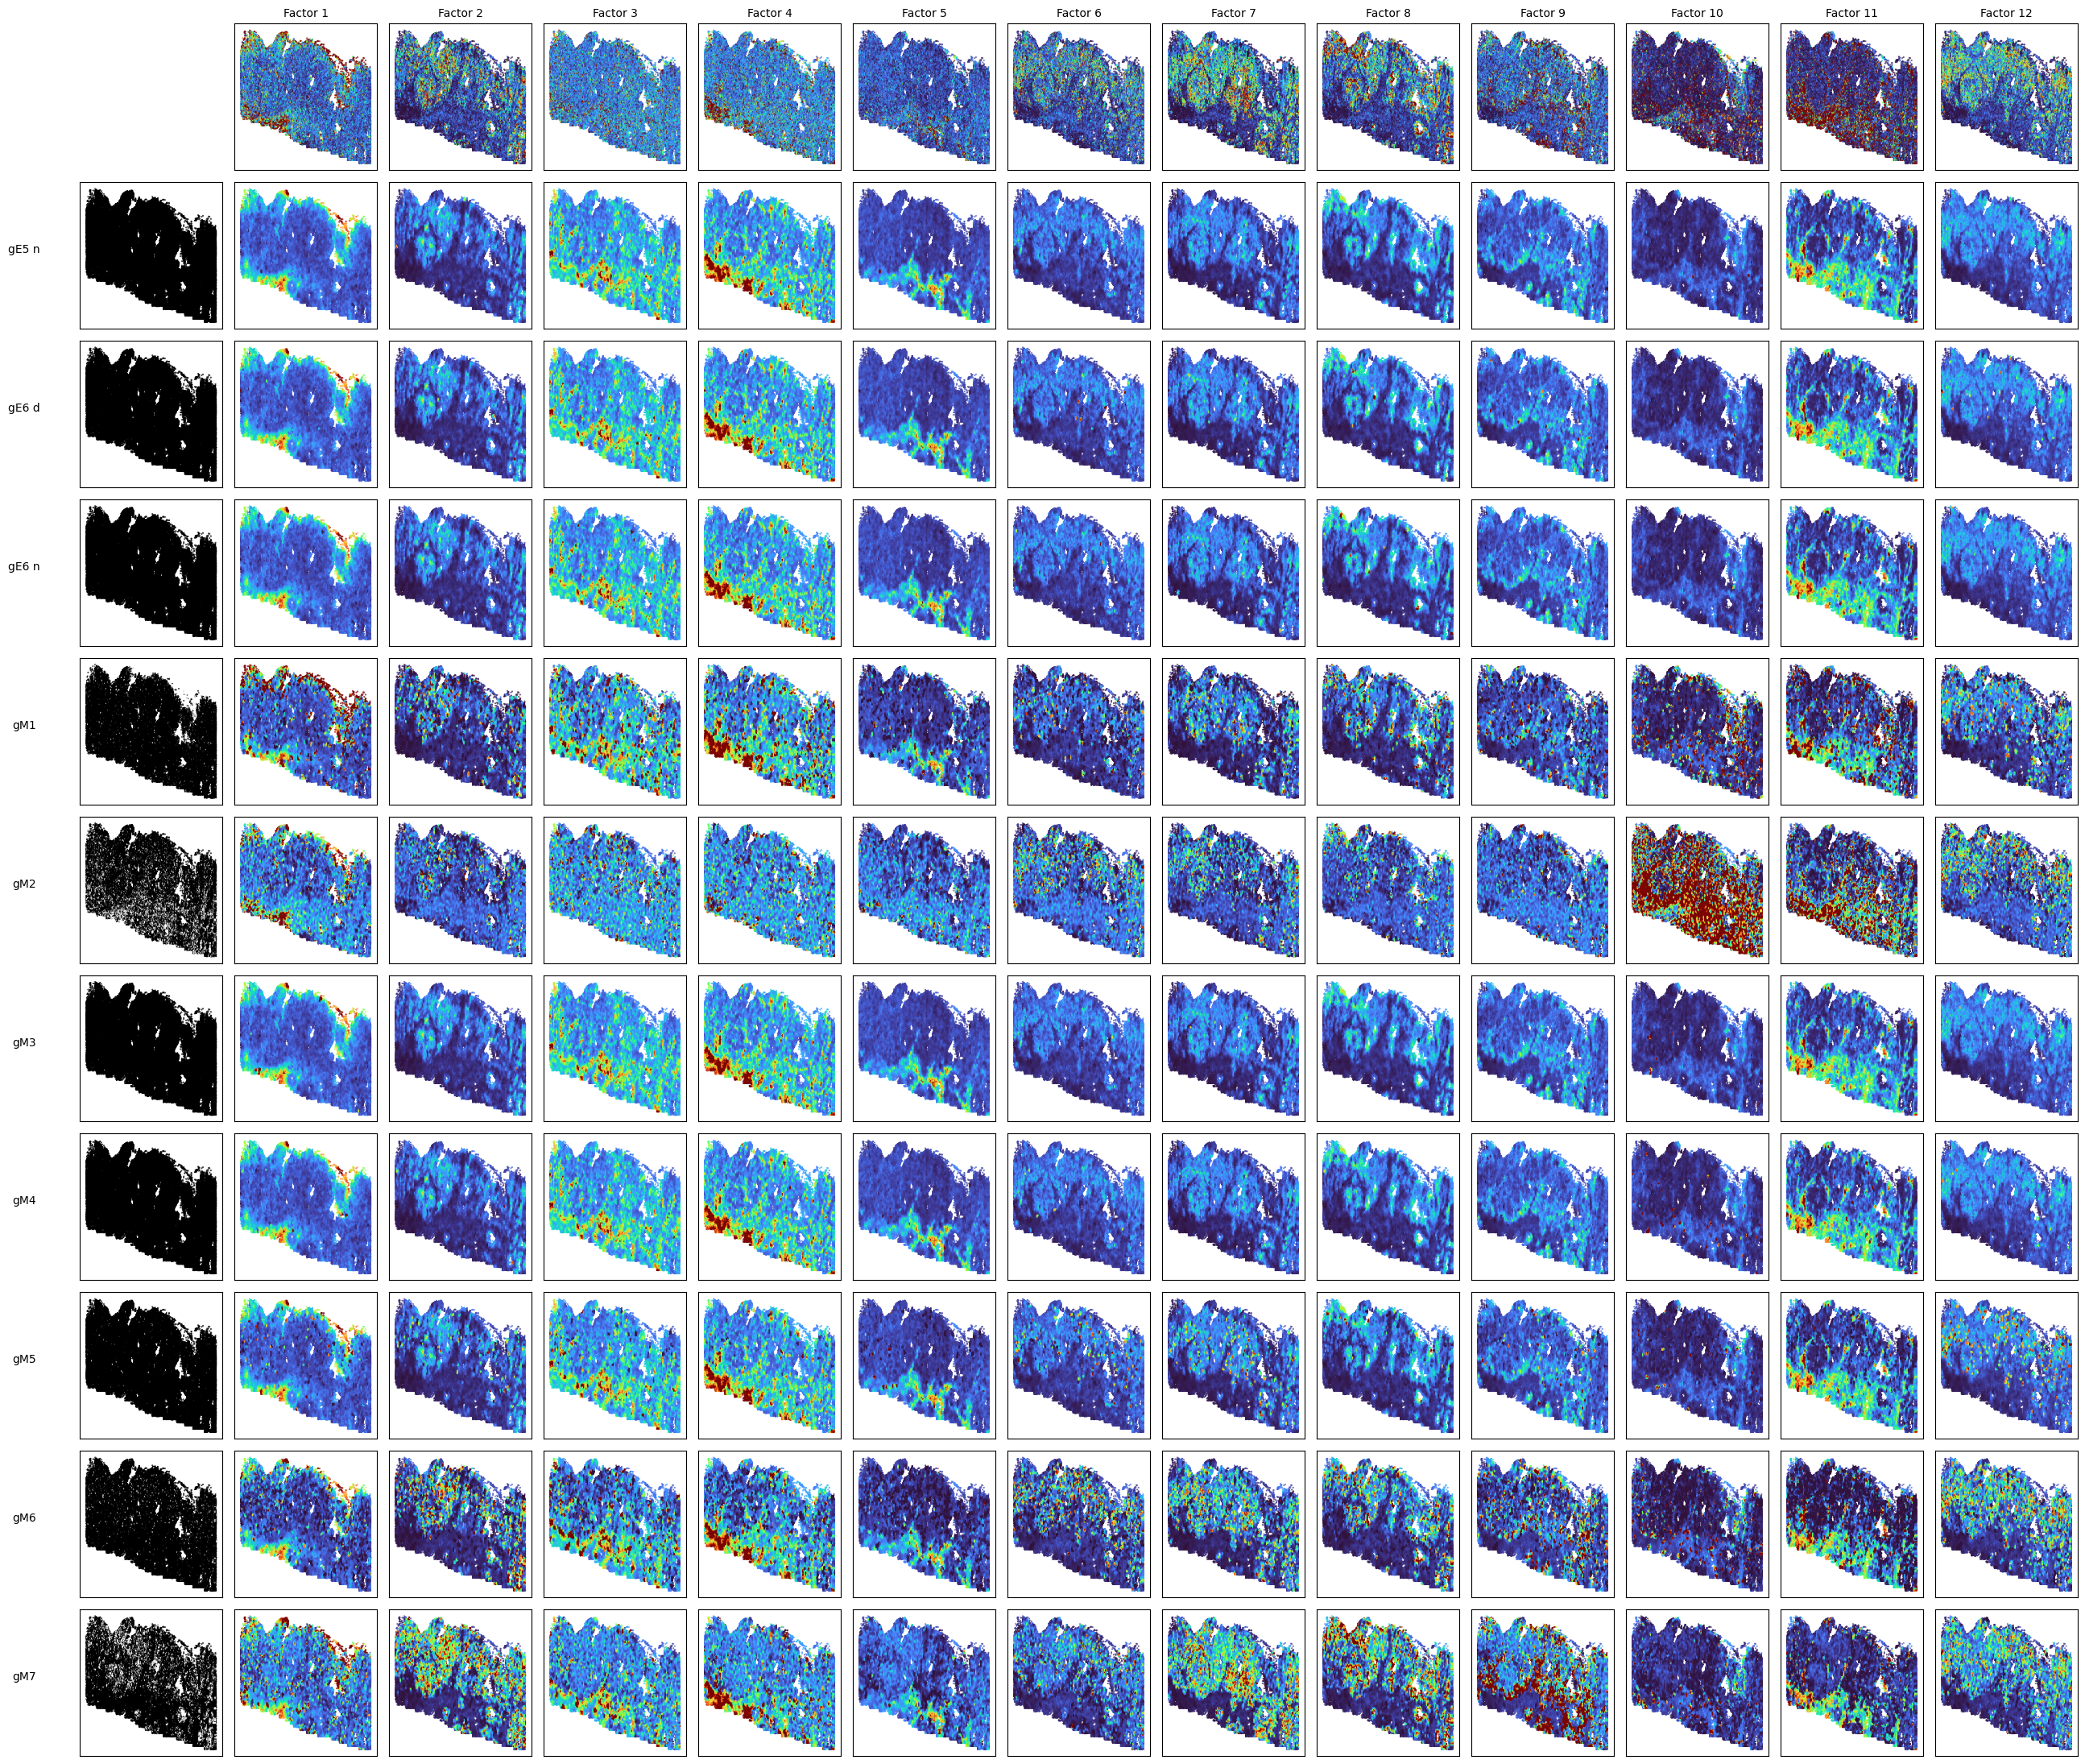
\includegraphics[width=0.98\linewidth]{MGGP_NSF_paper/HuColonCa-FFPE/posterior_2.png}
\caption{{\bf MERFISH CRC slices to show results from NSF versus MGNSF.}XXX }
\label{fig4b}
\end{figure}

\begin{figure}[!h]
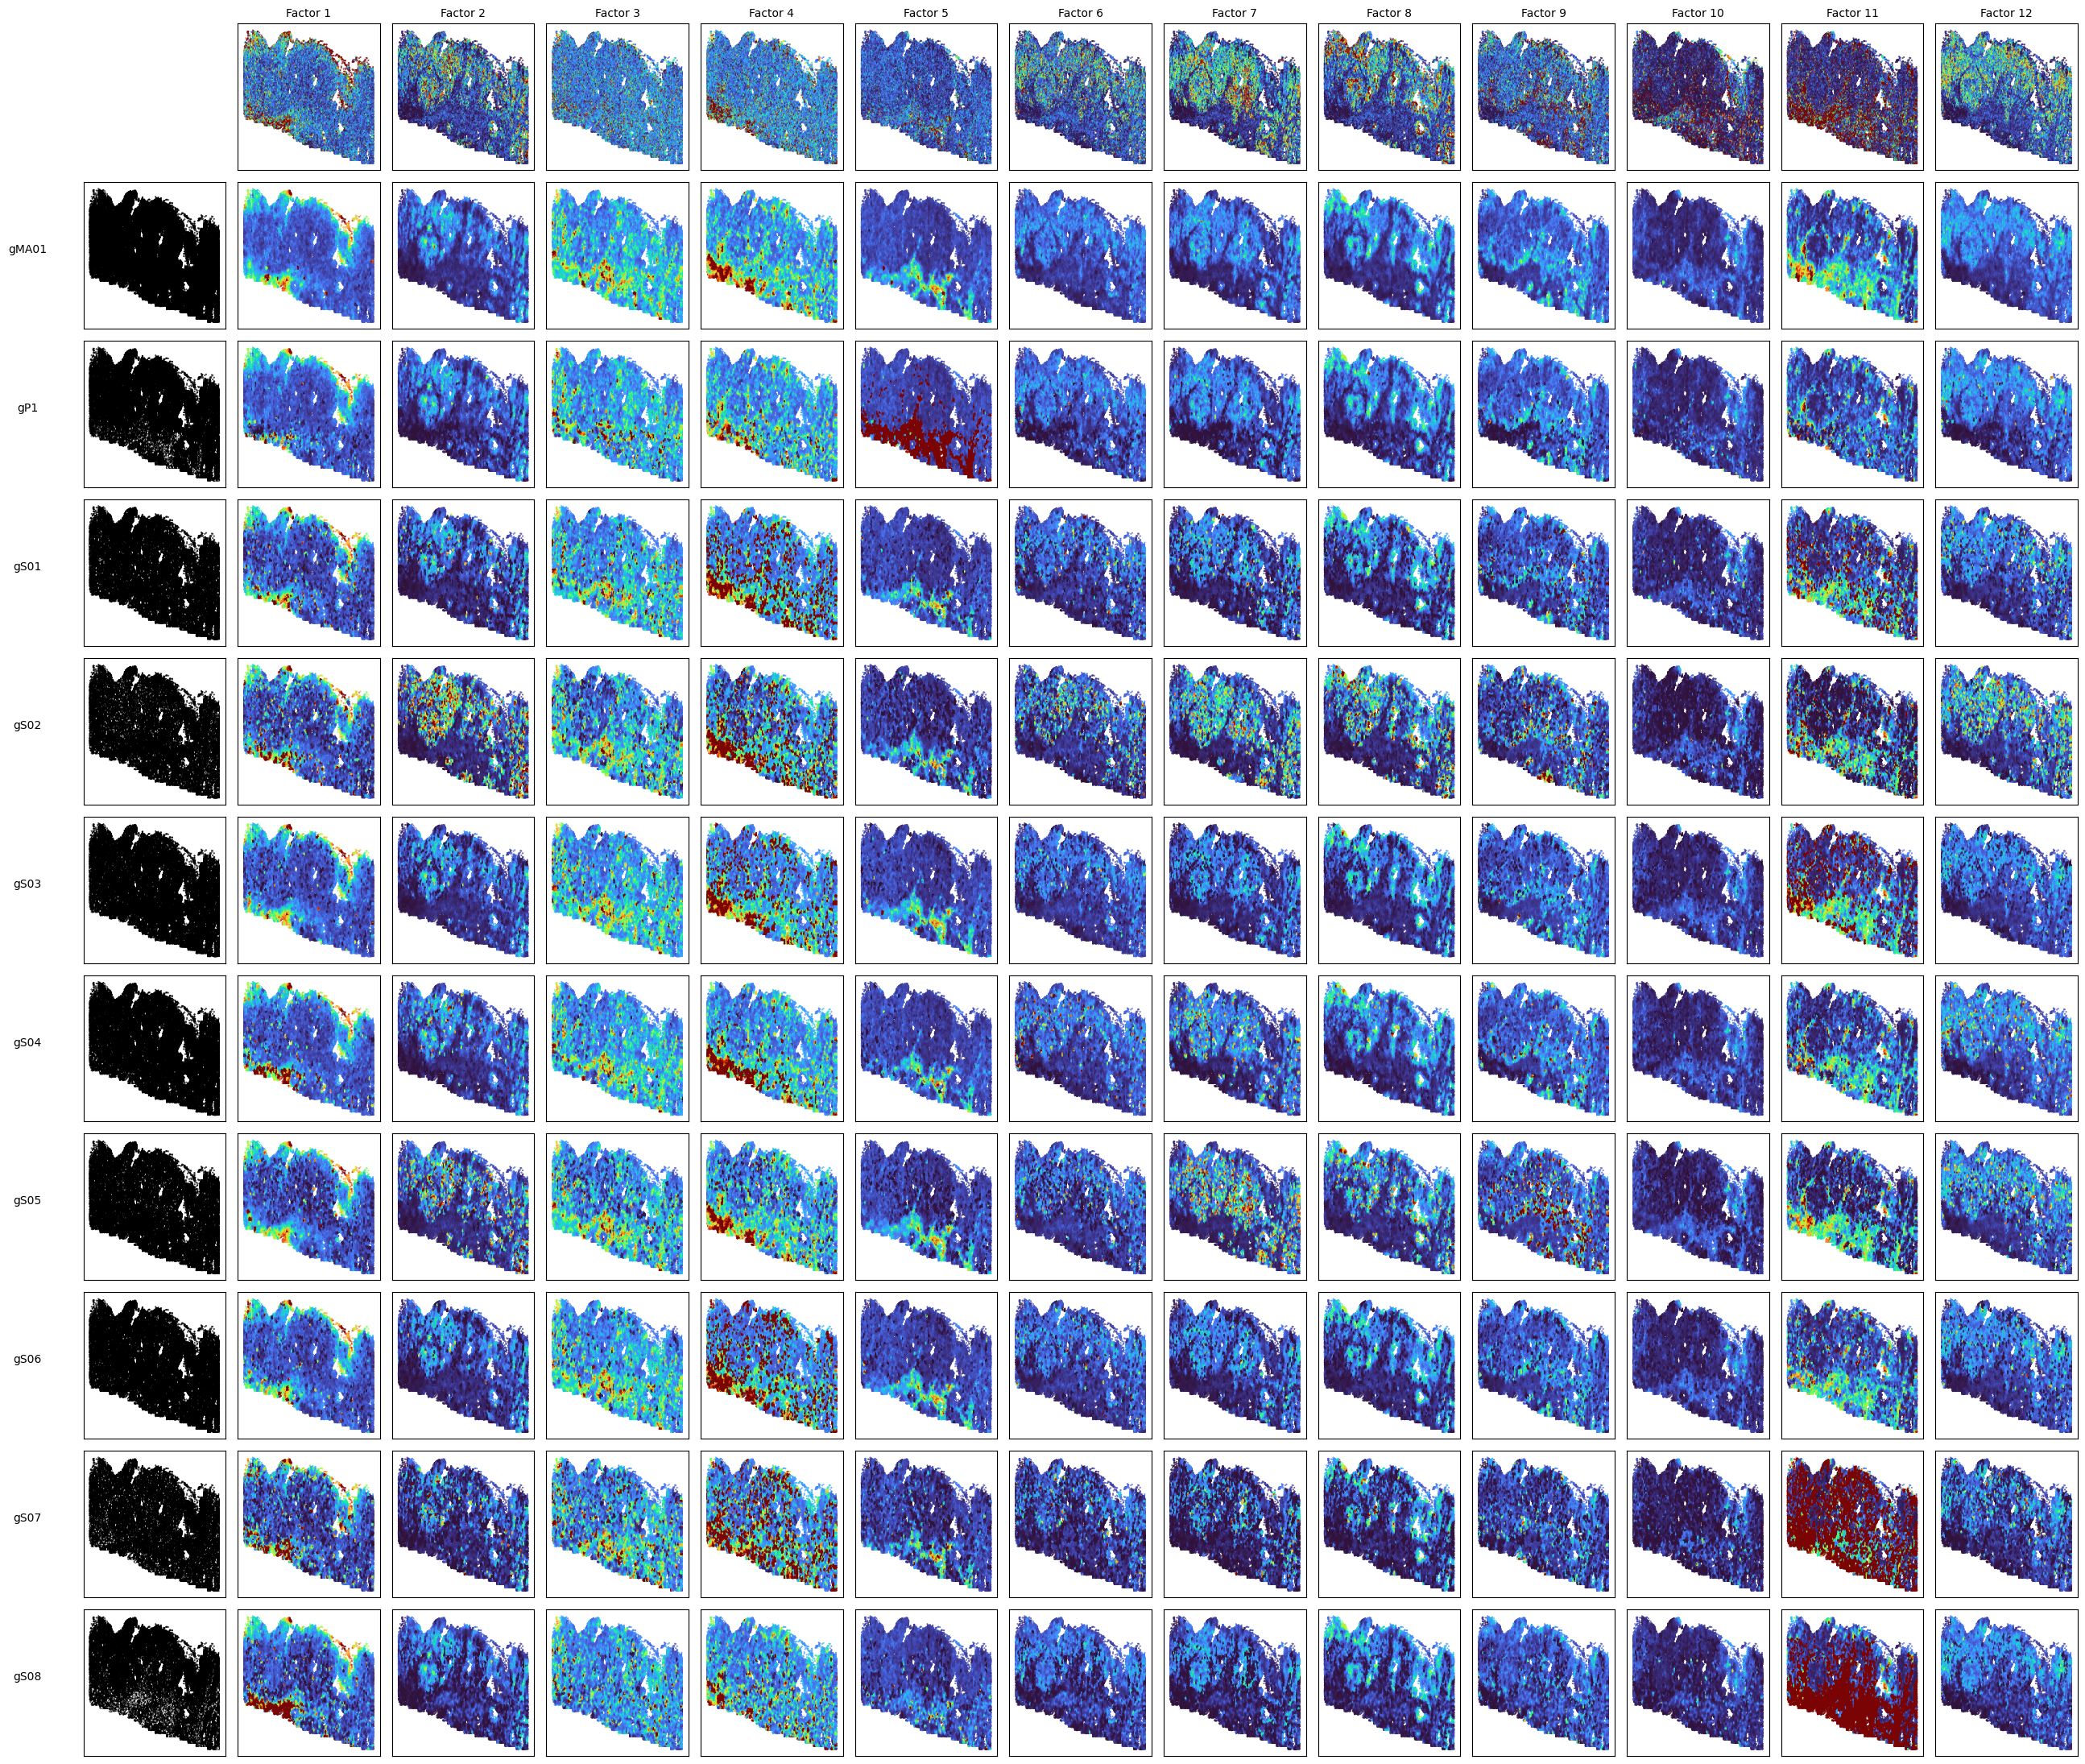
\includegraphics[width=0.98\linewidth]{MGGP_NSF_paper/HuColonCa-FFPE/posterior_3.png}
\caption{{\bf MERFISH CRC slices to show results from NSF versus MGNSF.}XXX }
\label{fig4c}
\end{figure}

\begin{figure}[!h]
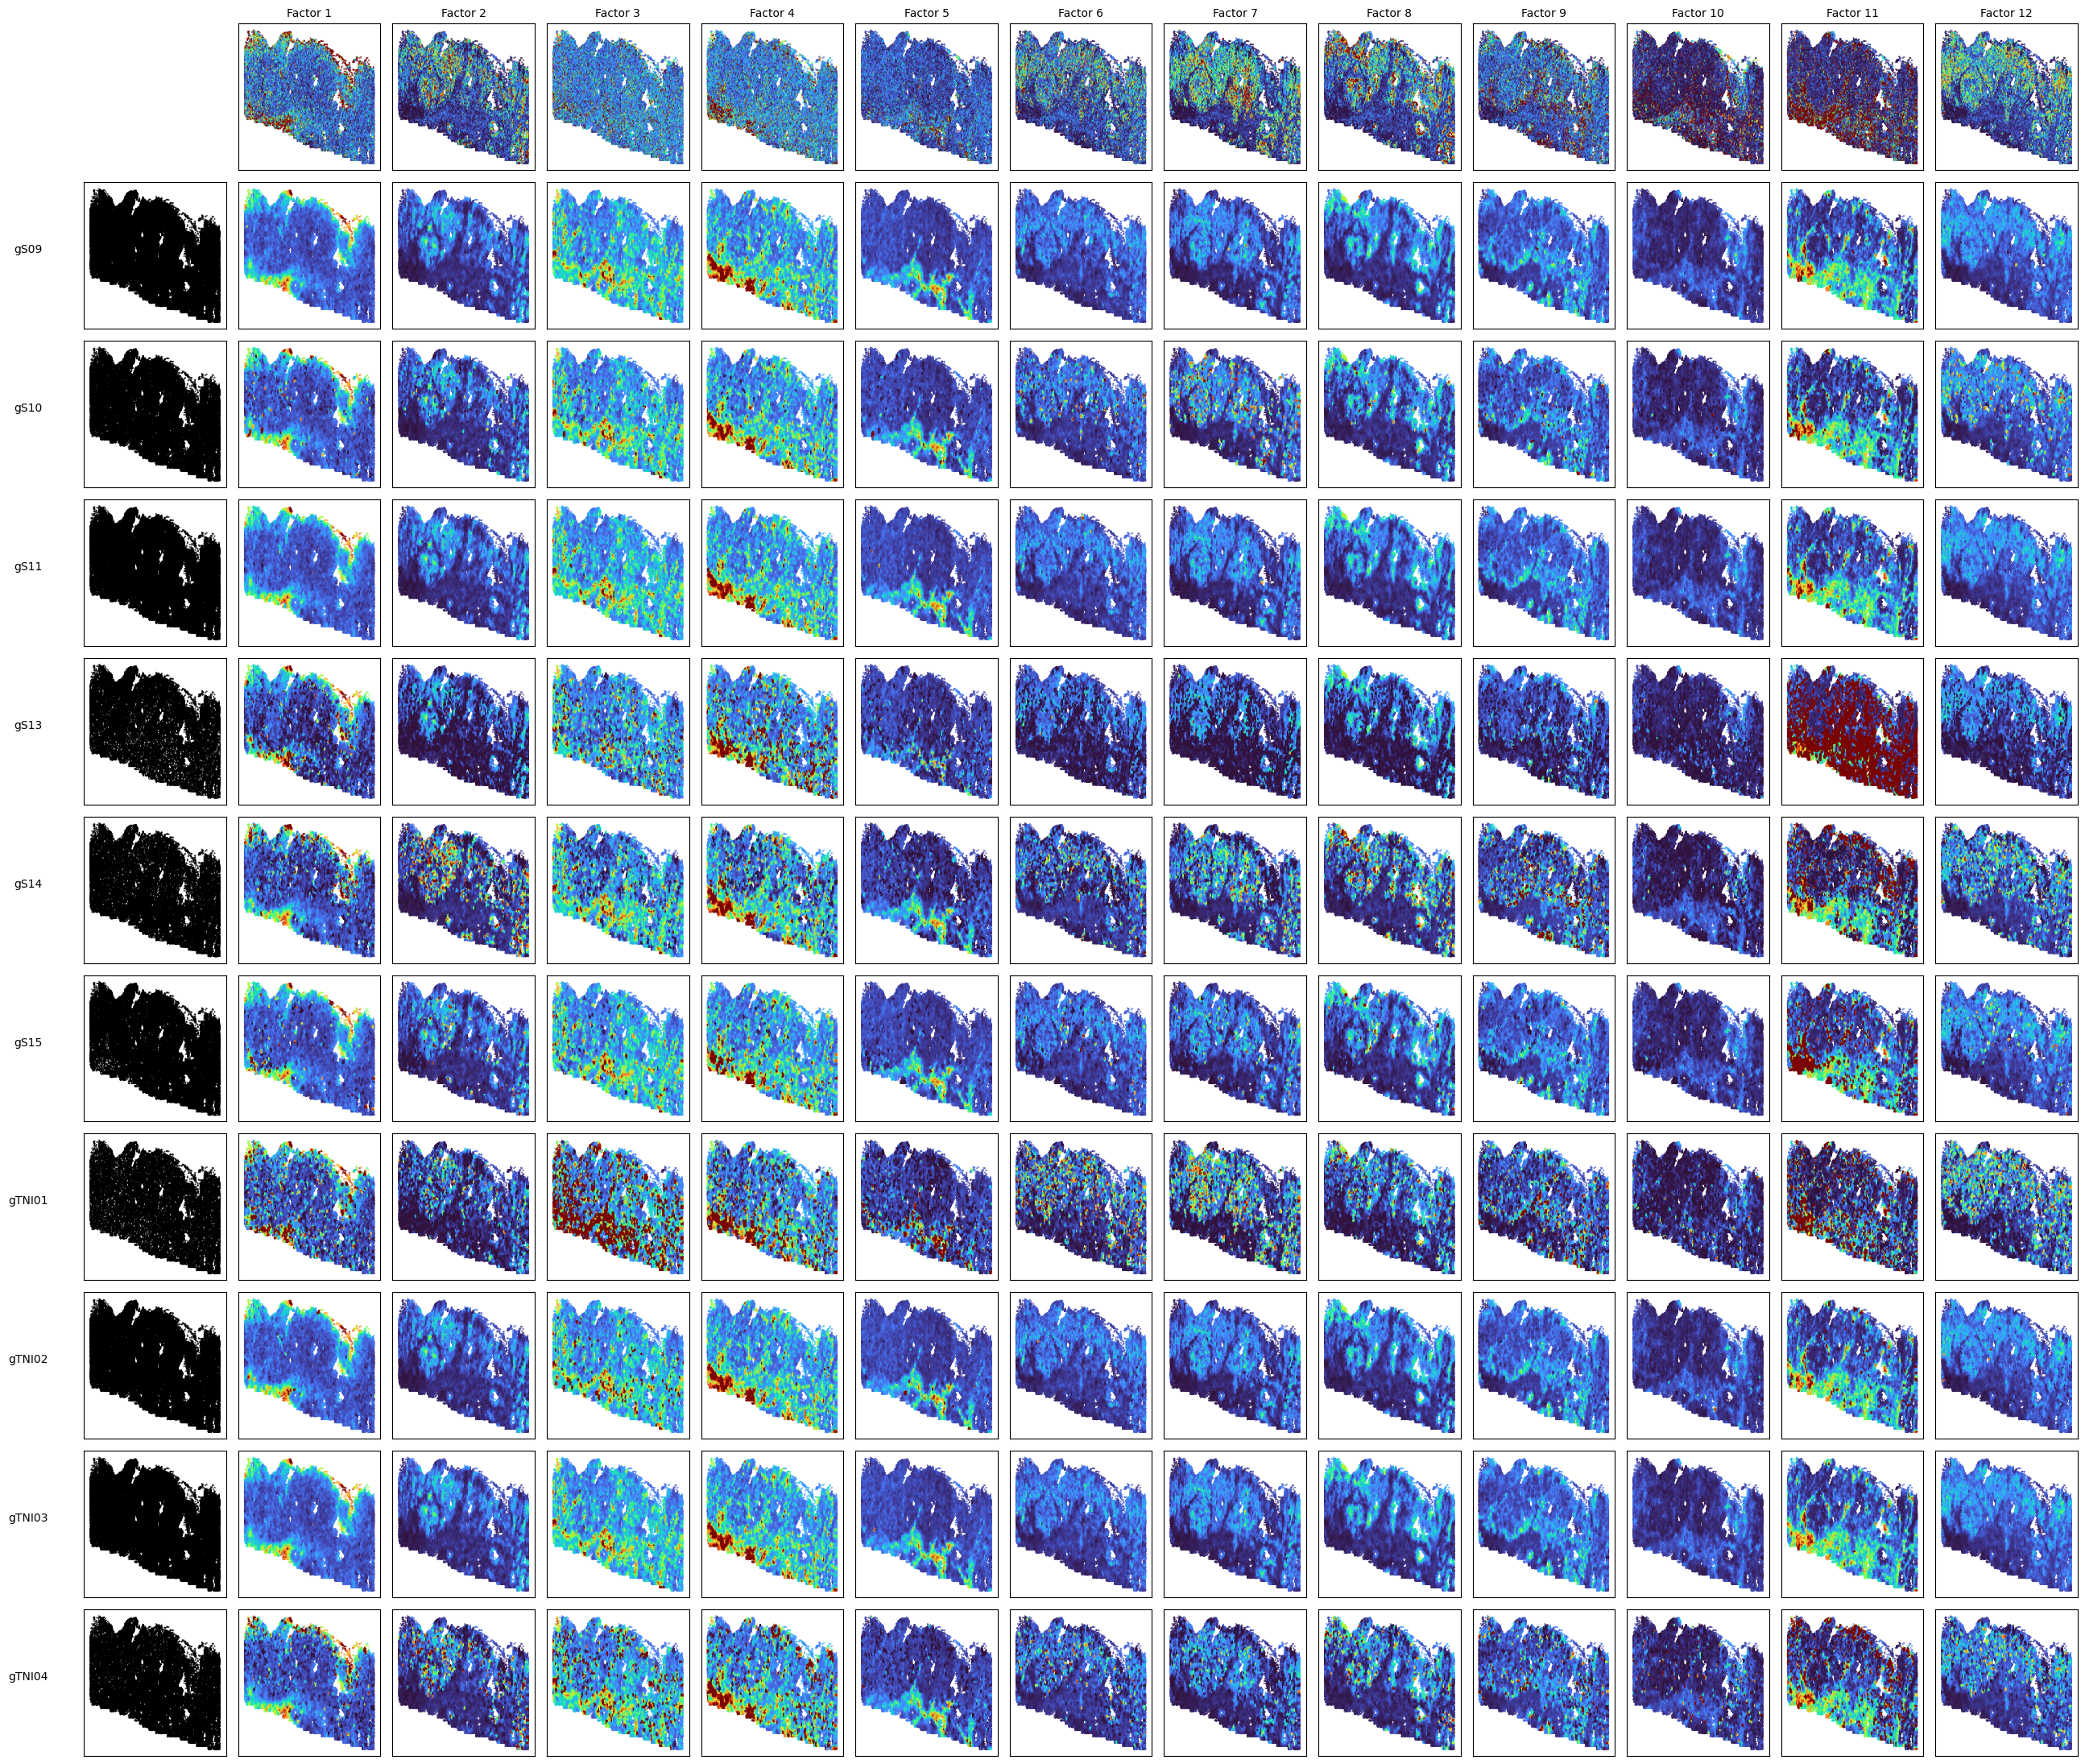
\includegraphics[width=0.98\linewidth]{MGGP_NSF_paper/HuColonCa-FFPE/posterior_4.png}
\caption{{\bf MERFISH CRC slices to show results from NSF versus MGNSF.}XXX }
\label{fig4d}
\end{figure}

\begin{figure}[!h]
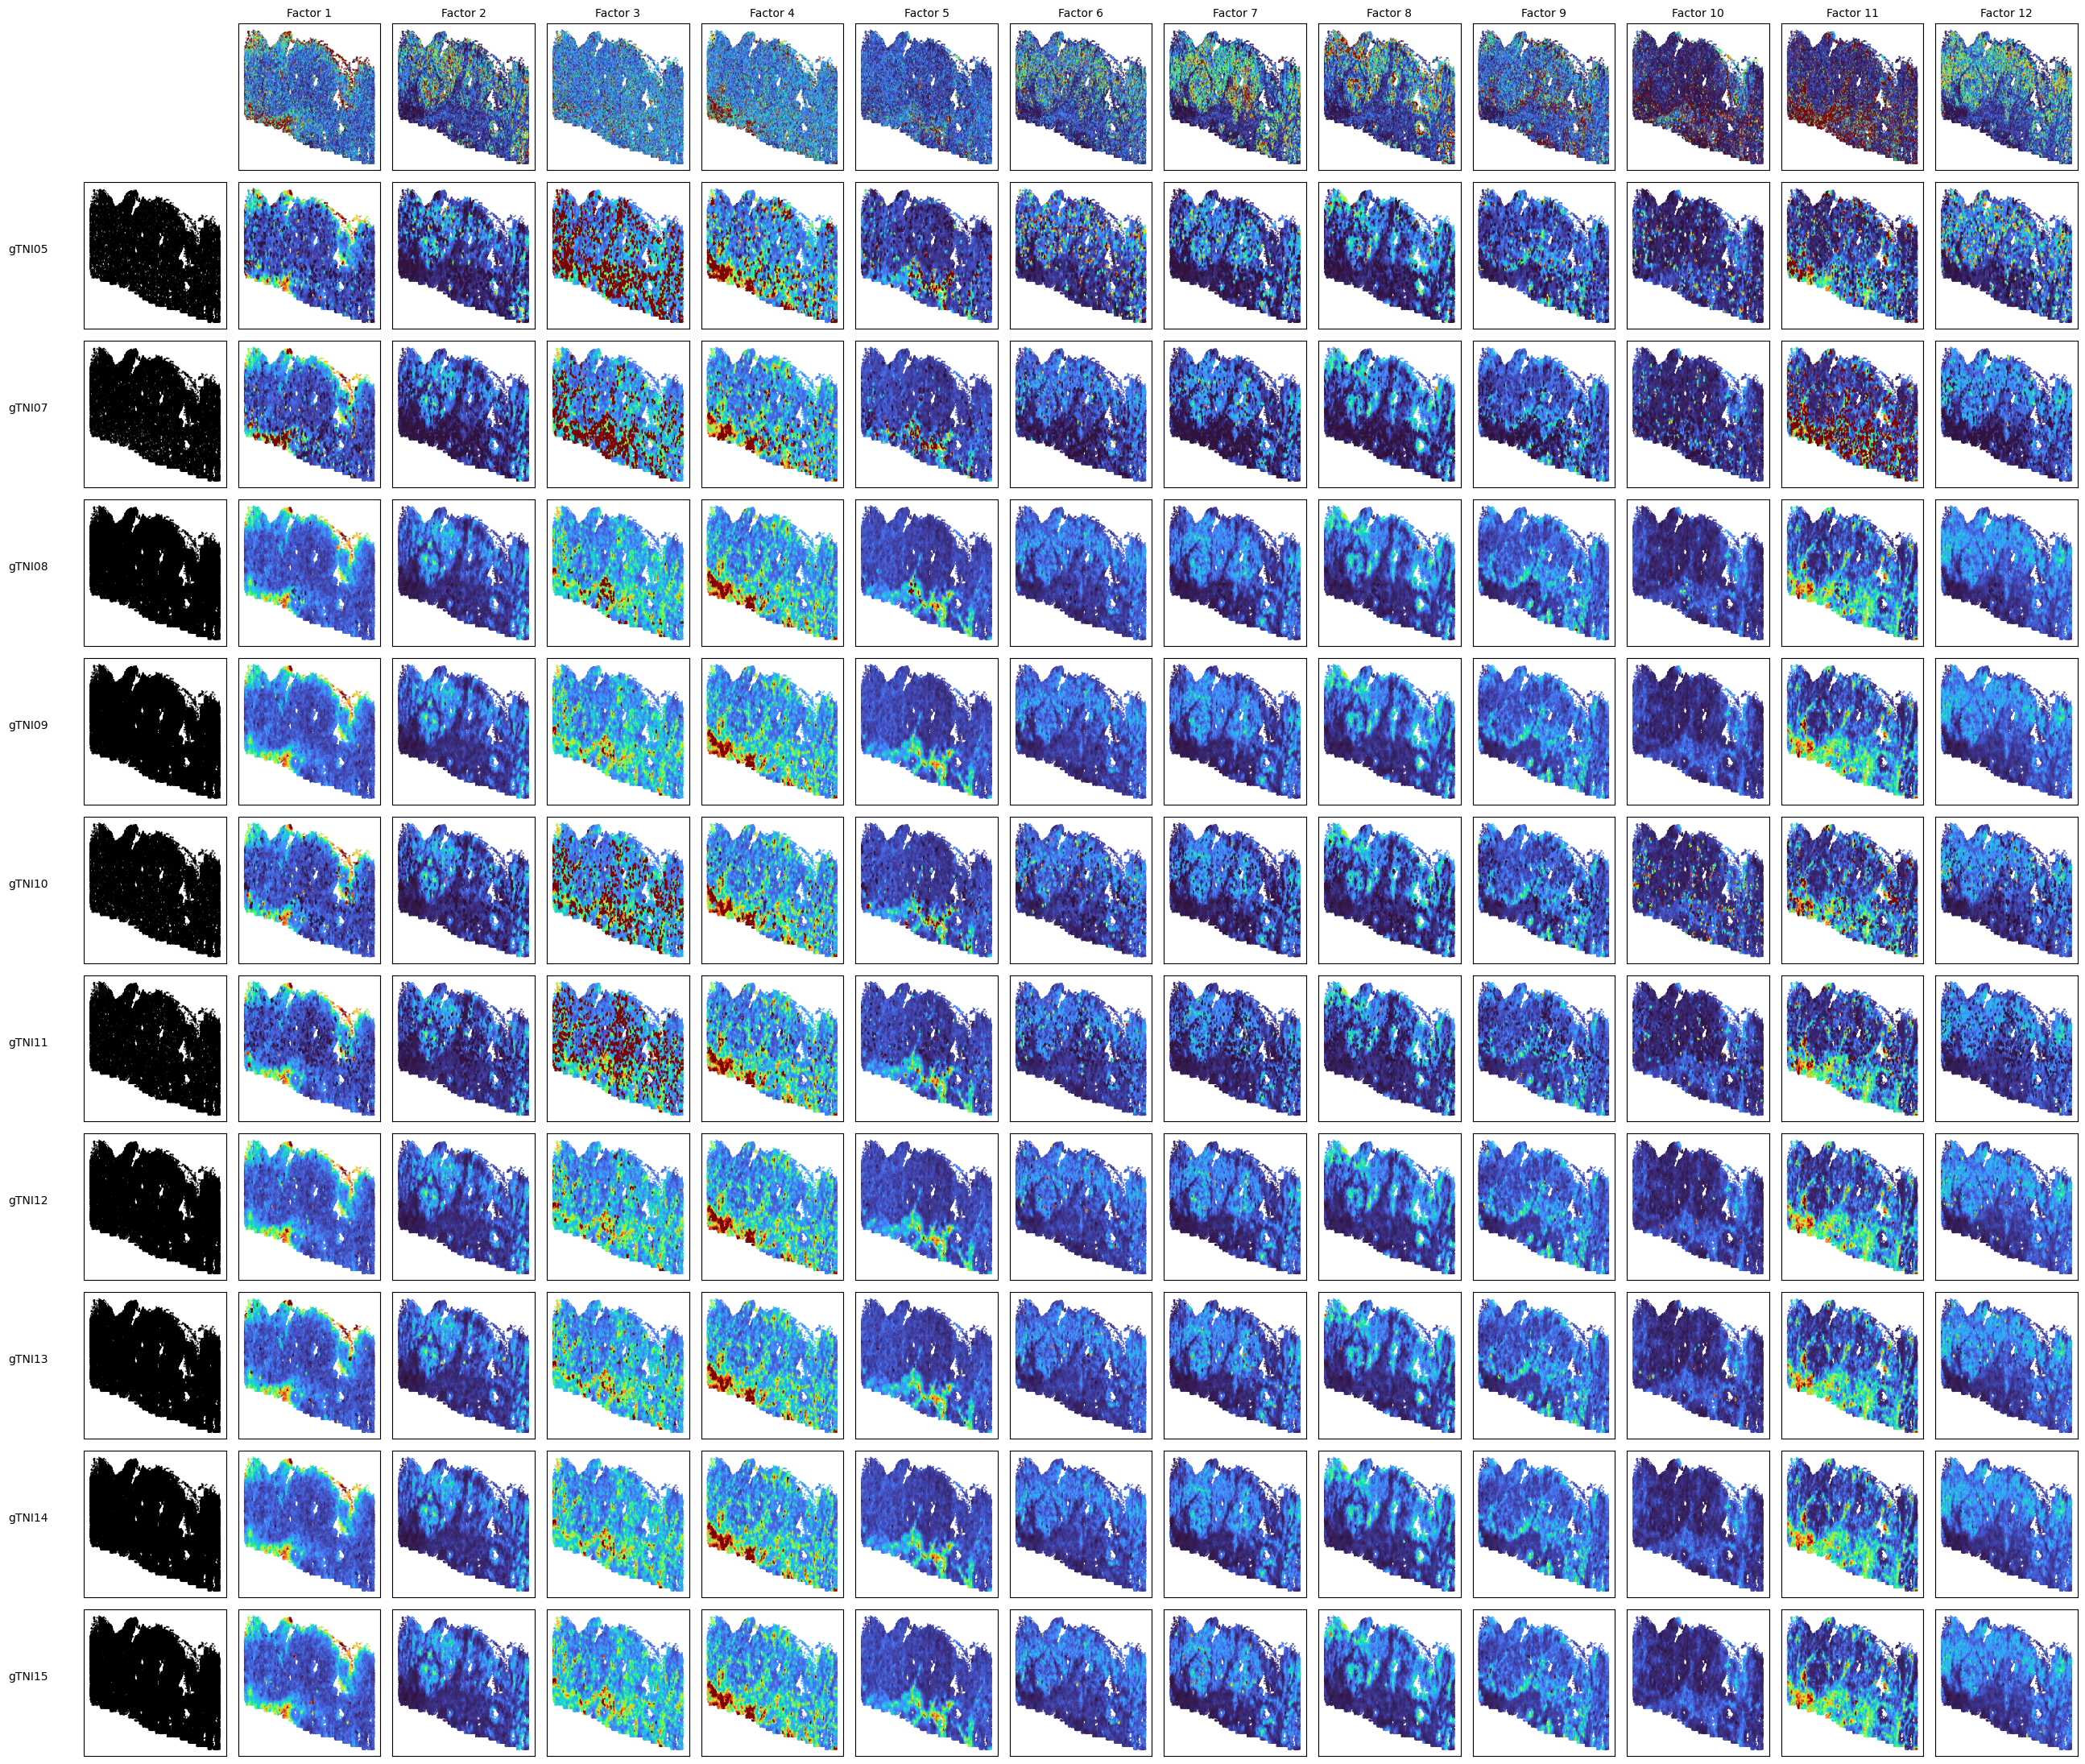
\includegraphics[width=0.98\linewidth]{MGGP_NSF_paper/HuColonCa-FFPE/posterior_5.png}
\caption{{\bf MERFISH CRC slices to show results from NSF versus MGNSF.}XXX }
\label{fig4e}
\end{figure}

\begin{figure}[!h]
\includegraphics[width=0.98\linewidth]{MGGP_NSF_paper/liver_fibrosis/factors.png}
\caption{{\bf MERFISH liver slices to show factors learned by the the VNNGP MGGP NSF} }
\label{fig7-liver}
\end{figure}

\begin{figure}[!h]
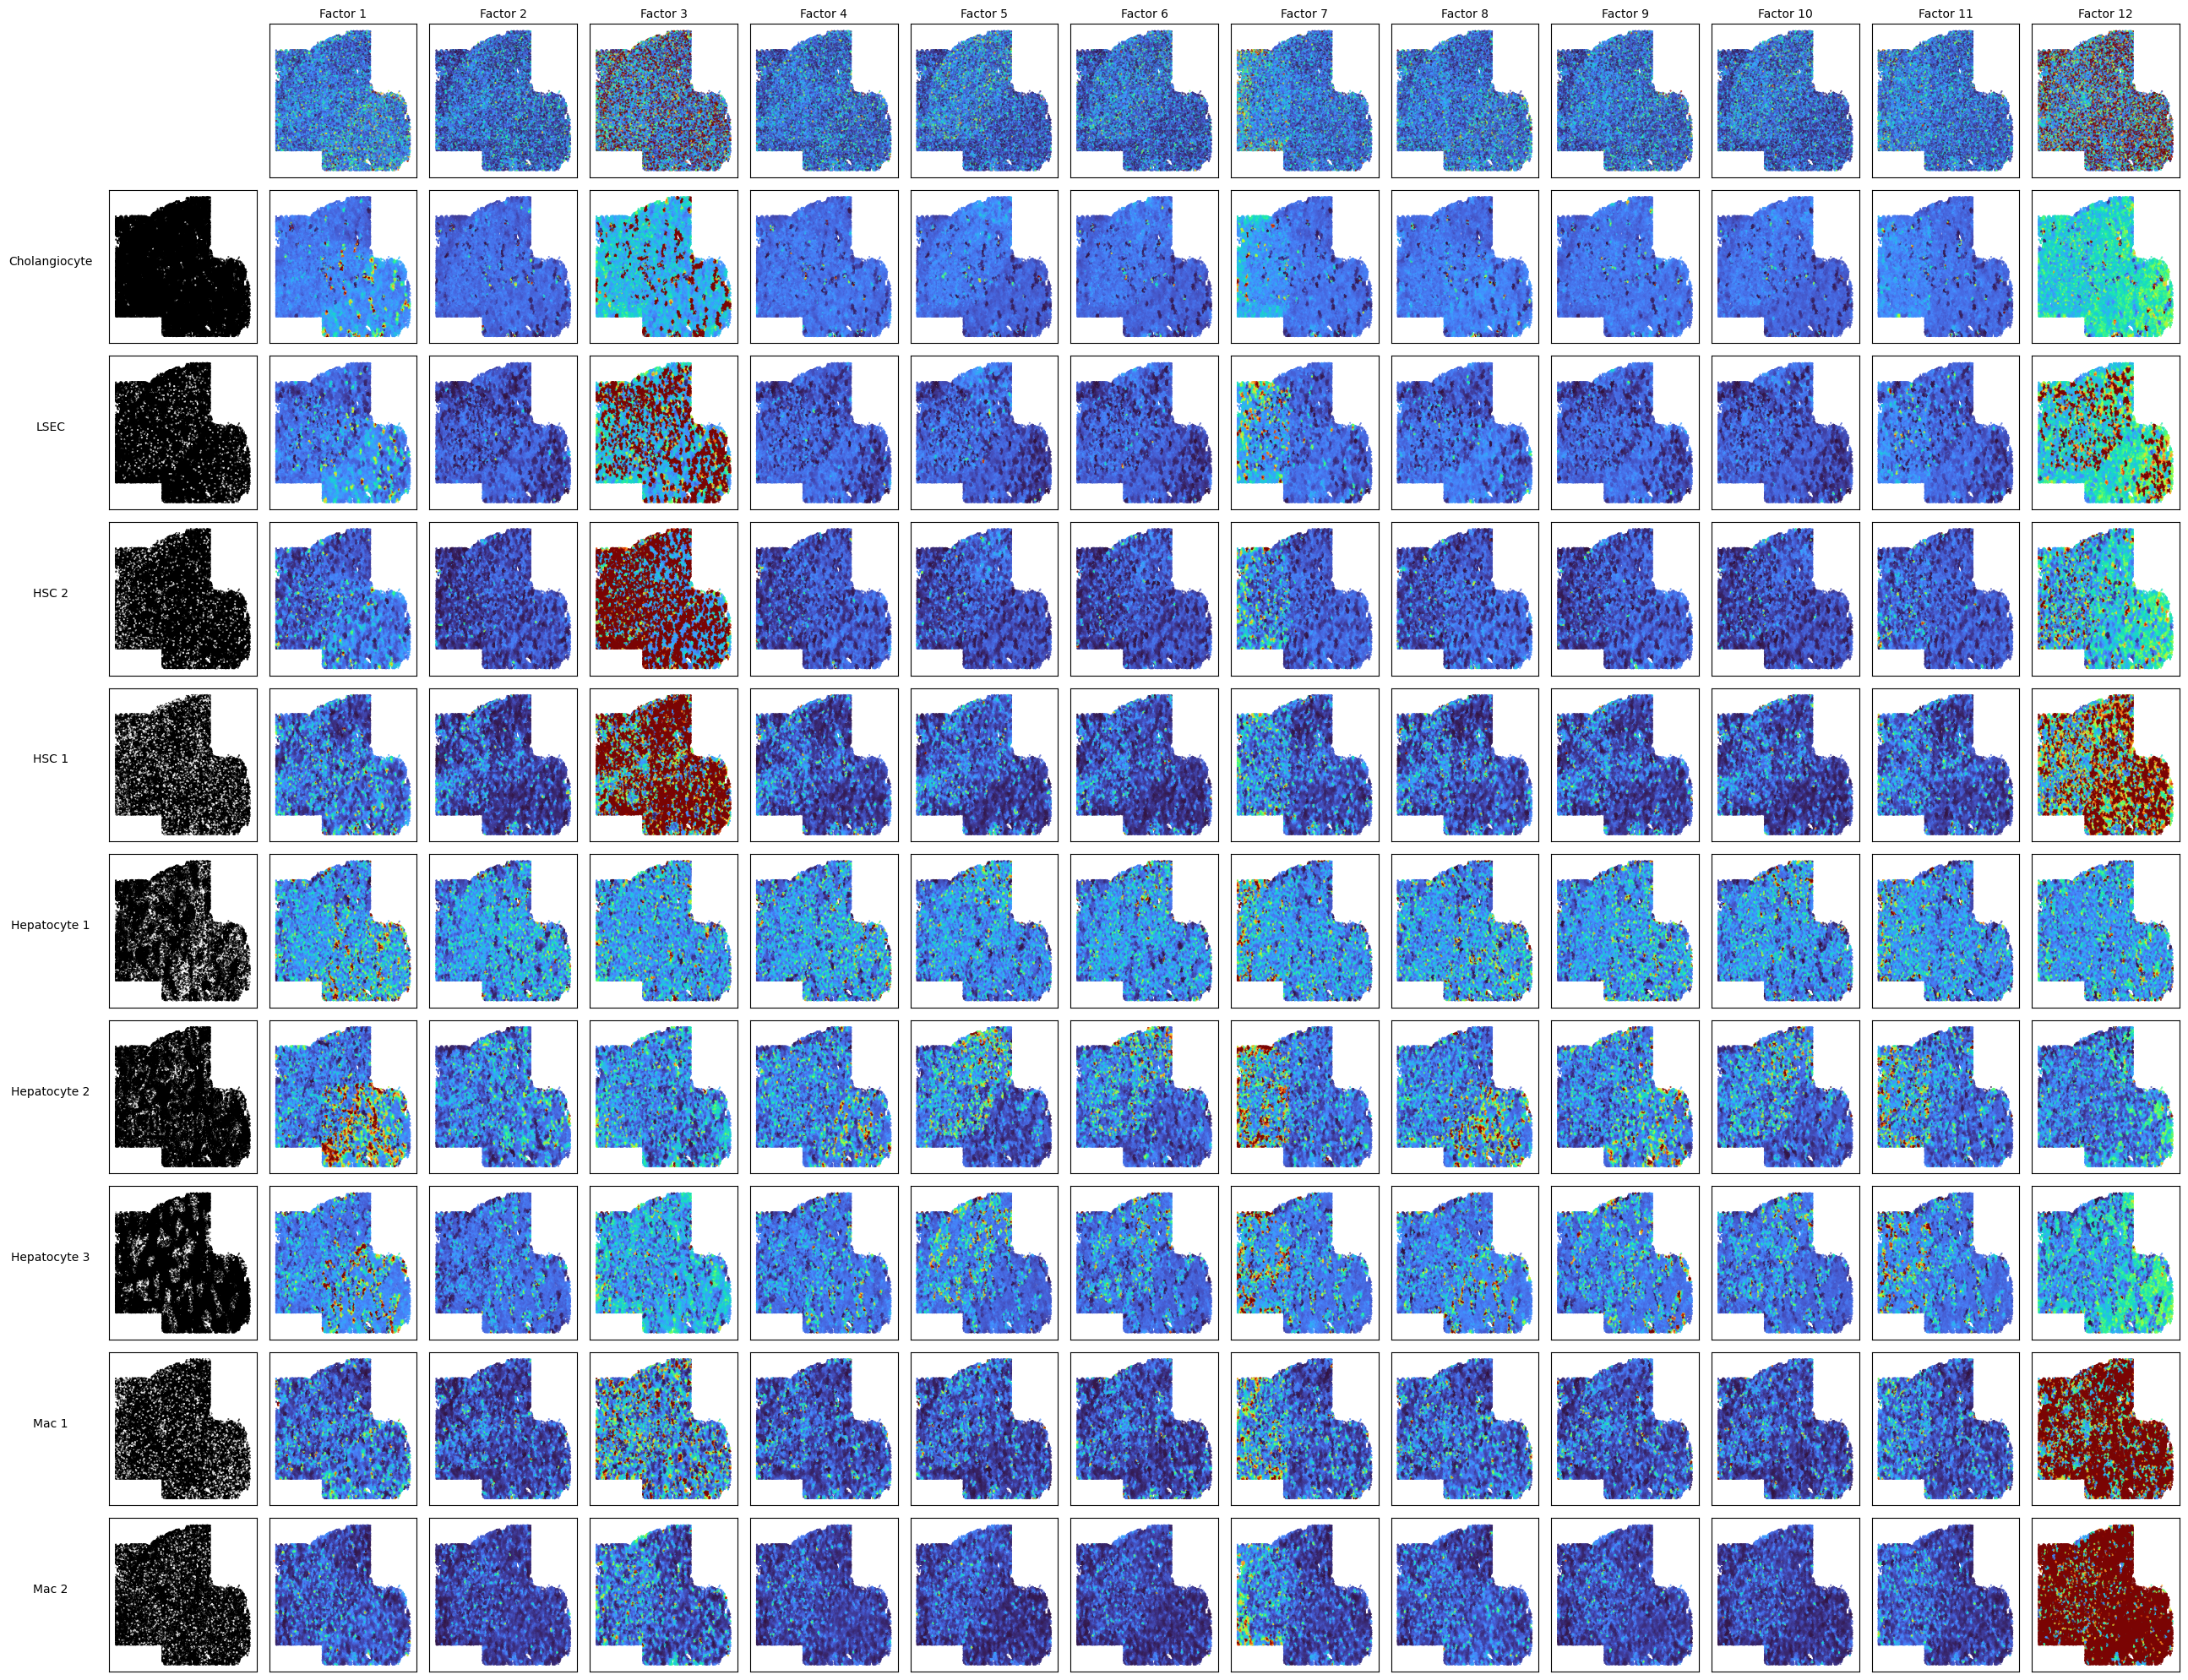
\includegraphics[width=0.98\linewidth]{MGGP_NSF_paper/liver_fibrosis/posteriors.png}
\caption{{\bf predictive conditional posteriors of MERFISH liver slices} }
\label{fig8-liver-posteriors}
\end{figure}

% ----------------------------
% (Optional) Slide-seqV2 hippocampus section moved out of main Results:
% [Placeholder: relocate the "Predictive posteriors reveal limitations of MGGP..." and
% "VNNGP improves local fidelity..." sections to Supplement if still desired.]
% ----------------------------
\clearpage





% Place figure captions after the first paragraph in which they are cited.
\begin{figure}[!h]
\caption{{\bf Bold the figure title.}
Figure caption text here, please use this space for the figure panel descriptions instead of using subfigure commands. A: Lorem ipsum dolor sit amet. B: Consectetur adipiscing elit.}
\label{fig1}
\end{figure}




\section*{Discussion}
Nulla mi mi, venenatis sed ipsum varius, Table~\ref{table1} volutpat euismod diam. Proin rutrum vel massa non gravida. Quisque tempor sem et dignissim rutrum. Lorem ipsum dolor sit amet, consectetur adipiscing elit. Morbi at justo vitae nulla elementum commodo eu id massa. In vitae diam ac augue semper tincidunt eu ut eros. Fusce fringilla erat porttitor lectus cursus, vel sagittis arcu lobortis. Aliquam in enim semper, aliquam massa id, cursus neque. Praesent faucibus semper libero~\cite{bib3}.

\section*{Conclusion}

CO\textsubscript{2} Maecenas convallis mauris sit amet sem ultrices gravida. Etiam eget sapien nibh. Sed ac ipsum eget enim egestas ullamcorper nec euismod ligula. Curabitur fringilla pulvinar lectus consectetur pellentesque. Quisque augue sem, tincidunt sit amet feugiat eget, ullamcorper sed velit. 

Sed non aliquet felis. Lorem ipsum dolor sit amet, consectetur adipiscing elit. Mauris commodo justo ac dui pretium imperdiet. Sed suscipit iaculis mi at feugiat. Ut neque ipsum, luctus id lacus ut, laoreet scelerisque urna. Phasellus venenatis, tortor nec vestibulum mattis, massa tortor interdum felis, nec pellentesque metus tortor nec nisl. Ut ornare mauris tellus, vel dapibus arcu suscipit sed. Nam condimentum sem eget mollis euismod. Nullam dui urna, gravida venenatis dui et, tincidunt sodales ex. Nunc est dui, sodales sed mauris nec, auctor sagittis leo. Aliquam tincidunt, ex in facilisis elementum, libero lectus luctus est, non vulputate nisl augue at dolor. For more information, see \nameref{S1_Appendix}.

\section*{Supporting information}


% Reset counters
\setcounter{section}{0}
\renewcommand\thesection{S\arabic{section}}


\section{Useful Identities}

In this section we display Gaussian marginalization and the computation of the KL divergence of two Gaussian distributions, both derived in Damianou et al. 2015 \cite{Damianou2015-dy} and Townes et al. 2023 \cite{Townes2023-it} respectively.
\subsection{Gaussian Marginalization}\label{subsecA1}

We start by defining the following distributions:
\[p(f|u) = \mathcal{N}(f| Wu, \Sigma_f)\]
\[p(u) = \mathcal{N}(u| m_u, \Sigma_u)\]

The marginal distribution becomes the following:

\[p(f) = \mathcal{N}(f| Wm_u, \Sigma_f+W\Sigma_{u}W^T)\]
\subsection{KL divergence}\label{subsecA2}

We define the following distributions, where $u \in \mathbb{R}^N$:

\[p(u) = \mathcal{N}(u| \mu, \Sigma)\]
\[q(u) = \mathcal{N}(u| m, S)\]

The closed form of the KL divergence over $q(u)$, becomes:


\[ \text{KL} \left( q(\mathbf{u}) \parallel p(\mathbf{u}) \right) = \frac{1}{2} \left[ \log \frac{|\Sigma|}{|S|} - N + \text{tr} \left\{ \Sigma^{-1} S \right\} + (m - \mu)' \Sigma^{-1} (m - \mu) \right] \]

\section{Locally Conditioned KL Approximation for Multivariate Gaussian Variational Inference}


We approximate the KL divergence between the variational distribution \( q(U) \) and the prior \( p(U) \) using a locally conditional chain rule factorization. Let \( U = [U_1, \dots, U_M] \) be the collection of inducing variables.






We begin by expanding the $p(U)$ prior using the chain rule:
\begin{align*}
p(U) &= p(U_M | U_{1, \dots, M-1}) p(U_{1, \dots, M-1}) \\
&= p(U_M | U_{1, \dots, M-1}) p(U_{M-1} | U_{1, \dots, M-2}) p(U_{1, \dots, M-2}) \\
&= p(U_1) \prod_{j=2}^{M} p(U_j | U_{1, \dots, j-1}).
\end{align*}

Under the local conditional approximation, this becomes:
\[
p(U) \approx \prod_{j=1}^{M} p(U_j | U_{n(j)}).
\]

Then, the variational distribution $q(U)$ can be expanded similarly:

\begin{align*}
q(U) &= q(U_1) \prod_{j=2}^{M} q(U_j | U_{1, \dots, j-1})\\
&\approx  \prod_{j=1}^{M} q(U_j | U_{n(j)})
\end{align*}



The KL divergence between $q(U)$ and $p(U)$ is given by:

\[
\mathrm{KL}(q(U) \| p(U)) = \mathbb{E}_{q(U)} \left[ \log \frac{q(U)}{p(U)} \right]
\]

Next, the log ratio can be expanded and approximated as the product of $M$ terms:

\[
\mathbb{E}_{q(U)} \left[ \log \frac{q(U)}{p(U)} \right] \approx \mathbb{E}_{q(U)} \left[ \log \prod_{j=1}^{M} \frac{q(U_j | U_{n(j)})}{p(U_j | U_{n(j)})} \right]
\]

Becoming a linear sum of expectations:

\[
= \mathbb{E}_{q(U)} \left[ \sum_{j=1}^{M} \log \frac{q(U_j | U_{n(j)})}{p(U_j | U_{n(j)})} \right]
\]

\[
= \sum_{j=1}^{M} \mathbb{E}_{q(U)} \left[ \log \frac{q(U_j | U_{n(j)})}{p(U_j | U_{n(j)})} \right]
\]

We then apply \textbf{Law of total expectation} which gives:

\[
= \sum_{j=1}^{M} \mathbb{E}_{q(U_{n(j)})} \left[ \mathbb{E}_{q(U_j| U_{n(j)})} \left[ \log \frac{q(U_j | U_{n(j)})}{p(U_j | U_{n(j)})} \right] \right]
\]


We assume that both the prior and variational posterior distributions over
\(U = [U_1, \dots, U_M]\) are multivariate Gaussian. In particular, we write

\[
p(U) = \mathcal{N}(U \mid 0,\, K),
\qquad
q(U) = \mathcal{N}(U \mid m,\, S),
\]

where \(K\) and \(S\) denote the prior and variational covariance matrices, and
\(m = [m_1, \dots, m_M]\) is the variational mean. Here we assume a zero-mean prior.

The conditional prior is given by:

\[
p(U_j | U_{n(j)}) = \mathcal{N}\left( K_{jn(j)} K_{n(j)n(j)}^{-1} U_{n(j)}, \; k_{jj} - K_{jn(j)} K_{n(j)n(j)}^{-1} K_{n(j)j} \right)
\]

The conditional variational distribution is given by:

\[
q(U_j | U_{n(j)}) = \mathcal{N}\left( m_j + S_{jn(j)} S_{n(j)n(j)}^{-1} (U_{n(j)} - m_{n(j)}), \; s_{jj} - S_{jn(j)} S_{n(j)n(j)}^{-1} S_{n(j)j} \right)
\]

\text{This reduces to }
$q(U_j) = \mathcal{N}(m_j, s_{jj})$ if  $s_{jj}$ is diagonal.\\ 

For notational compactness in subsequent expressions, we define these conditionals:

\begin{align*}
p(U_j | U_{n(j)}) &= \mathcal{N}\left( \beta_j^\top U_{n(j)}, \; \tau_j^2 \right) \\
q(U_j | U_{n(j)}) &= \mathcal{N}\left( m_j + \alpha_j^\top (U_{n(j)} - m_{n(j)}), \; \tilde{\tau}_j^2 \right)
\end{align*}

Where:

\begin{align*}
\beta_j^\top &= K_{jn(j)} K_{n(j)n(j)}^{-1}, \quad
\tau_j^2 = k_{jj} - K_{jn(j)} K_{n(j)n(j)}^{-1} K_{n(j)j} \\
\alpha_j^\top &= S_{jn(j)} S_{n(j)n(j)}^{-1}, \quad
\tilde{\tau}_j^2 = s_{jj} - S_{jn(j)} S_{n(j)n(j)}^{-1} S_{n(j)j}
\end{align*}

The KL divergence between two univariate Gaussians is:

\begin{align*}
\mathrm{KL}(q \,\|\, p)
&= \frac{1}{2} \left[
\log \frac{s_p^2}{s_q^2}
+ \frac{s_q^2}{s_p^2}
+ \frac{(\mu_q - \mu_p)^2}{s_p^2}
- 1
\right].
\end{align*}


The KL between $q(U_j | U_{n(j)})$ and $p(U_j | U_{n(j)})$ is given by:

\begin{align*}
\mathrm{KL}\!\left(q(U_j \mid U_{n(j)}) \,\|\, p(U_j \mid U_{n(j)})\right)
&= \frac{1}{2} \Bigg[
\log \frac{\tau_j^2}{\tilde{\tau}_j^2}
+ \frac{\tilde{\tau}_j^2}{\tau_j^2}
+ \frac{\big(m_j + \alpha_j^\top (U_{n(j)} - m_{n(j)}) - \beta_j^\top U_{n(j)}\big)^2}{\tau_j^2}
- 1 \Bigg].
\end{align*}


Then we calculate the expectation of this KL under $q(U_{n(j)})$:

\[
\Rightarrow \mathbb{E}_{q(U_{n(j)})} \left[ \mathrm{KL} \left( q(U_j | U_{n(j)}) \| p(U_j | U_{n(j)}) \right) \right]
\]

\begin{align*}
= \frac{1}{2} \left[
\log \frac{\tau_j^2}{\tilde{\tau}_j^2}
+ \frac{\tilde{\tau}_j^2}{\tau_j^2}
+ \frac{\mathbb{E}_{q(U_{n(j)})}\!\left[
\left(m_j + \alpha_j^\top (U_{n(j)} - m_{n(j)}) - \beta_j^\top U_{n(j)}\right)^2
\right]}{\tau_j^2}
- 1 \right].
\end{align*}



We treat the mean term:
\[
\left(m_j + \alpha_j^\top (U_{n(j)} - m_{n(j)}) - \beta_j^\top U_{n(j)}\right)^2
\]

This is rewritten as:
\[
= \left((\alpha_j - \beta_j)^\top U_{n(j)} + (m_j - \alpha_j^\top m_{n(j)})\right)^2
\]

Using the following identity:
\[
\mathbb{E}_{x \sim \mathcal{N}(\mu, \Sigma)} \left[(a^\top x + b)^2\right] = a^\top \Sigma a + (a^\top \mu + b)^2
\]

Applying this gives:

\begin{align*}
\mathbb{E}_{q(U_{n(j)})}\!\left[
\left(m_j + \alpha_j^\top (U_{n(j)} - m_{n(j)}) - \beta_j^\top U_{n(j)}\right)^2
\right]
=
(\alpha_j - \beta_j)^\top S_{n(j)n(j)} (\alpha_j - \beta_j)
\\
\quad + \left[\,(\alpha_j - \beta_j)^\top m_{n(j)} + \left(m_j - \alpha_j^\top m_{n(j)}\right)\right]^2.
\end{align*}


This expectation can be expanded further and simplified as:

\[
= \alpha_j^\top S_{n(j)n(j)} \alpha_j + \beta_j^\top S_{n(j)n(j)} \beta_j - 2 \alpha_j^\top S_{n(j)n(j)} \beta_j + (\beta_j^\top m_{n(j)} - m_j)^2
\]

Substituting this into the KL formula yields the final approximation:



\begin{align*}
   \mathrm{KL}(q(U) \| p(U)) \approx \sum_{j=1}^{M} \mathbb{E}_{q(U_{n(j)})} \left[ \mathbb{E}_{q(U_j| U_{n(j)})} \left[ \log \frac{q(U_j | U_{n(j)})}{p(U_j | U_{n(j)})} \right] \right]
\end{align*}


\begin{align*}
= \sum_{j=1}^{M} \frac{1}{2} \Bigg[
&\log \frac{\tau_j^2}{\tilde{\tau}_j^2}
+ \frac{\tilde{\tau}_j^2}{\tau_j^2}
+ \frac{\left(m_j - \beta_j^\top m_{n(j)}\right)^2}{\tau_j^2} \\
&\quad + \frac{\beta_j^\top S_{n(j)n(j)} \beta_j}{\tau_j^2}
+ \frac{\alpha_j^\top S_{n(j)n(j)} \alpha_j}{\tau_j^2}
- \frac{2 \alpha_j^\top S_{n(j)n(j)} \beta_j}{\tau_j^2}
- 1
\Bigg].
\end{align*}


This decomposition allows for scalable computation of the KL divergence in sparse MGGP models using only local neighbor subsets \( n(j) \). It is especially useful for variational nearest-neighbor Gaussian processes (VNNGPs), and can be efficiently computed in parallel across all nodes.

% Include only the SI item label in the paragraph heading. Use the \nameref{label} command to cite SI items in the text.
\paragraph*{S1 Fig.}
\label{S1_Fig}
{\bf Bold the title sentence.} Add descriptive text after the title of the item (optional).

\paragraph*{S2 Fig.}
\label{S2_Fig}
{\bf Lorem ipsum.} Maecenas convallis mauris sit amet sem ultrices gravida. Etiam eget sapien nibh. Sed ac ipsum eget enim egestas ullamcorper nec euismod ligula. Curabitur fringilla pulvinar lectus consectetur pellentesque.

\paragraph*{S1 File.}
\label{S1_File}
{\bf Lorem ipsum.}  Maecenas convallis mauris sit amet sem ultrices gravida. Etiam eget sapien nibh. Sed ac ipsum eget enim egestas ullamcorper nec euismod ligula. Curabitur fringilla pulvinar lectus consectetur pellentesque.

\paragraph*{S1 Video.}
\label{S1_Video}
{\bf Lorem ipsum.}  Maecenas convallis mauris sit amet sem ultrices gravida. Etiam eget sapien nibh. Sed ac ipsum eget enim egestas ullamcorper nec euismod ligula. Curabitur fringilla pulvinar lectus consectetur pellentesque.

\paragraph*{S1 Appendix.}
\label{S1_Appendix}
{\bf Lorem ipsum.} Maecenas convallis mauris sit amet sem ultrices gravida. Etiam eget sapien nibh. Sed ac ipsum eget enim egestas ullamcorper nec euismod ligula. Curabitur fringilla pulvinar lectus consectetur pellentesque.

\paragraph*{S1 Table.}
\label{S1_Table}
{\bf Lorem ipsum.} Maecenas convallis mauris sit amet sem ultrices gravida. Etiam eget sapien nibh. Sed ac ipsum eget enim egestas ullamcorper nec euismod ligula. Curabitur fringilla pulvinar lectus consectetur pellentesque.

\section*{Acknowledgments}
Cras egestas velit mauris, eu mollis turpis pellentesque sit amet. Interdum et malesuada fames ac ante ipsum primis in faucibus. Nam id pretium nisi. Sed ac quam id nisi malesuada congue. Sed interdum aliquet augue, at pellentesque quam rhoncus vitae.

\nolinenumbers

% Either type in your references using
% \begin{thebibliography}{}
% \bibitem{}
% Text
% \end{thebibliography}
%
% or
%
% Compile your BiBTeX database using our plos2015.bst
% style file and paste the contents of your .bbl file
% here. See http://journals.plos.org/plosone/s/latex for 
% step-by-step instructions.
% 


\bibliography{paperpile}      % ← no .bib extension here



\end{document}

